\documentclass[11pt]{article}
\usepackage[margin = 1in]{geometry}
\usepackage{amsmath}
\usepackage{amssymb}
\usepackage{amsthm} % for proof environment
\usepackage{enumitem}
\usepackage{graphicx}
\usepackage{indentfirst}
\usepackage{caption}
\usepackage{lscape}
\usepackage{multirow}
\usepackage{array}
\usepackage{subcaption} % caption the subfigures
\usepackage{setspace}
\usepackage[round]{natbib}

\renewcommand{\labelenumii}{\alph*)}
\newcommand{\w}{\omega}
\newcommand{\p}{\prime}
\newcommand{\one}{\mathbf{1}}
\newcommand{\onep}{\mathbf{1}^\prime}
\newcommand{\lagr}{\mathcal{L}}
\newcommand{\inv}[1]{#1^{-1}}
\newcommand{\ev}{\mathbb{E}}
\renewcommand{\wp}{\omega^\prime}


\begin{document}

\begin{flushleft}
	Nick Hoffman \\
	Finance I, Spring 2020 A \\
	Assignment 2 \\
\end{flushleft}

\begin{enumerate}
	\item Because the market portfolio $ \w^m $ is a convex combination of efficient portfolios, it is itself efficient. Thus, it solves the portfolio problem:
	%
	\begin{gather*}
	\min_\w \frac{1}{2}\w^\p V \w \\
	\text{s.t.} \\
	\w^\p \bar{R} \geq \mu \\
	\w^\p \one = 1
	\end{gather*}
	
	The first-order condition for this problem is 
	\begin{equation}\label{foc1}
	\bar{R} = \frac{1}{\lambda_1} V \w^m - \frac{\lambda_2}{\lambda_1} \one 
	\end{equation}
	To derive the CAPM, I use (\ref{foc1}) twice. First, premultiply (\ref{foc1}) by $ \w^m $, yielding
	\begin{equation}\label{premult1}
	\bar{R}^m = \frac{1}{\lambda_1} \sigma^2_m - \frac{\lambda_2}{\lambda_1}
	\end{equation}
	where $\bar{R}^m$ is the return on the market portfolio. Now, introduce $ \w^z $, the ``zero-$ \beta $'' portfolio, which is constructed such that $ \w^{z\p}V \w^m  $ = 0; that is, $ \w^z $ is orthogonal to the market portfolio. Premultiplying (\ref{foc1}) by $ \w^z $ yields
	\begin{equation}\label{premult2}
	\bar{R} = -\frac{\lambda_2}{\lambda_1} 
	\end{equation}
	Substituting (\ref{premult2}) into (\ref{premult1}) gives
	\begin{equation}\label{premult3}
	\frac{1}{\lambda_1} = \frac{\bar{R}^m - \bar{R}^z}{\sigma_m^2}
	\end{equation}
	Substituting (\ref{premult2}) and (\ref{premult3}) into (\ref{foc1}) gives the CAPM:
	\[\bar{R} = \bar{R}^z \one + [\bar{R}^m - \bar{R}^z]\frac{V\w^m}{\sigma_m^2}\]
	For any asset $ n $ in the market portfolio, this result implies that
	\[\bar{R}_n = \bar{R}^z  + [\bar{R}^m - \bar{R}^z]\frac{cov(R_n, R_m)}{\sigma_m^2}\]
	
	\item To test the CAPM, I use the specification 
	\[r_i(t) = \hat{\alpha}_i + \hat{\beta}_i r_m(t) + \hat{\varepsilon}_t\]
	where $ r_i(t) $ is the return on asset $ i $ in period $ t $, and $ r_m(t) $ is the market return in period $ t $. I then test the null hypothesis that $ \hat{\alpha}_i = 0 $, and reject the null hypothesis if the resulting $ p $-value is less than 0.05. 
	\begin{enumerate}
		\item The results are reported in Table \ref{table_1_capm} \newpage
		
			\begin{table}[!htbp] \centering 
			\footnotesize
			\caption{} 
			\label{table_1_capm} 
			\begin{tabular}{@{\extracolsep{5pt}} cccc} 
				\\[-1.8ex]\hline 
				\hline \\[-1.8ex] 
				Industry & $ \beta $ & $ \alpha $ & $ p_\alpha $ \\ 
				\hline \\[-1.8ex] 
				Aero & $1.148$ & $0.001$ & $0.604$ \\ 
				Agric & $0.878$ & $$-$0.0004$ & $0.848$ \\ 
				Autos & $1.153$ & $$-$0.003$ & $0.102$ \\ 
				Banks & $1.077$ & $$-$0.0004$ & $0.800$ \\ 
				Beer & $0.736$ & $0.003$ & $0.075$ \\ 
				BldMt & $1.185$ & $$-$0.001$ & $0.498$ \\ 
				Books & $1.072$ & $$-$0.002$ & $0.177$ \\ 
				Boxes & $0.979$ & $0.0002$ & $0.919$ \\ 
				BusSv & $1.160$ & $$-$0.001$ & $0.348$ \\ 
				Chems & $1.048$ & $$-$0.00005$ & $0.969$ \\ 
				Chips & $1.415$ & $$-$0.002$ & $0.250$ \\ 
				Clths & $1.113$ & $$-$0.0001$ & $0.933$ \\ 
				Cnstr & $1.289$ & $$-$0.003$ & $0.071$ \\ 
				Coal & $1.160$ & $$-$0.005$ & $0.173$ \\ 
				Drugs & $0.783$ & $0.002$ & $0.112$ \\ 
				ElcEq & $1.218$ & $0.0002$ & $0.904$ \\ 
				FabPr & $1.106$ & $$-$0.004$ & $0.058$ \\ 
				Fin & $1.240$ & $$-$0.0003$ & $0.793$ \\ 
				Food & $0.667$ & $0.003$ & $0.026$ \\ 
				Fun & $1.371$ & $0.0004$ & $0.826$ \\ 
				Gold & $0.608$ & $$-$0.003$ & $0.419$ \\ 
				Guns & $0.821$ & $0.003$ & $0.114$ \\ 
				Hardw & $1.231$ & $$-$0.003$ & $0.134$ \\ 
				Hlth & $1.133$ & $$-$0.002$ & $0.484$ \\ 
				Hshld & $0.790$ & $0.0003$ & $0.788$ \\ 
				Insur & $0.961$ & $0.001$ & $0.407$ \\ 
				LabEq & $1.323$ & $$-$0.002$ & $0.324$ \\ 
				Mach & $1.243$ & $$-$0.001$ & $0.259$ \\ 
				Meals & $1.034$ & $0.0004$ & $0.810$ \\ 
				MedEq & $0.896$ & $0.002$ & $0.264$ \\ 
				Mines & $1.121$ & $$-$0.002$ & $0.457$ \\ 
				Oil & $0.813$ & $0.0005$ & $0.780$ \\ 
				Other & $1.176$ & $$-$0.007$ & $0.0003$ \\ 
				Paper & $0.969$ & $$-$0.00004$ & $0.977$ \\ 
				PerSv & $1.095$ & $$-$0.005$ & $0.011$ \\ 
				RlEst & $1.255$ & $$-$0.007$ & $0.002$ \\ 
				Rtail & $1.008$ & $0.001$ & $0.447$ \\ 
				Rubbr & $1.081$ & $$-$0.0004$ & $0.787$ \\ 
				Ships & $1.117$ & $$-$0.001$ & $0.742$ \\ 
				Smoke & $0.645$ & $0.005$ & $0.017$ \\ 
				Soda & $0.820$ & $0.002$ & $0.418$ \\ 
				Softw & $1.591$ & $$-$0.006$ & $0.057$ \\ 
				Steel & $1.337$ & $$-$0.005$ & $0.005$ \\ 
				Telcm & $0.789$ & $0.001$ & $0.429$ \\ 
				Toys & $1.175$ & $$-$0.003$ & $0.079$ \\ 
				Trans & $1.065$ & $$-$0.001$ & $0.625$ \\ 
				Txtls & $1.158$ & $$-$0.002$ & $0.320$ \\ 
				Util & $0.501$ & $0.002$ & $0.114$ \\ 
				Whlsl & $1.048$ & $$-$0.001$ & $0.635$ \\ 
				\hline \\[-1.8ex] 
		\end{tabular} 
	\end{table} 
		

For most industries, we cannot reject the null hypothesis that $\hat{\alpha} = 0$. The $ p $-value is only below the critical value of 0.05 for seven industries in the table. 
	
	\item Figure (\ref{q2_fmtest}) shows the Fama-Macbeth test: 
	
	\begin{figure}[!ht]
		\centering
		\caption{}
		\label{q2_fmtest}
		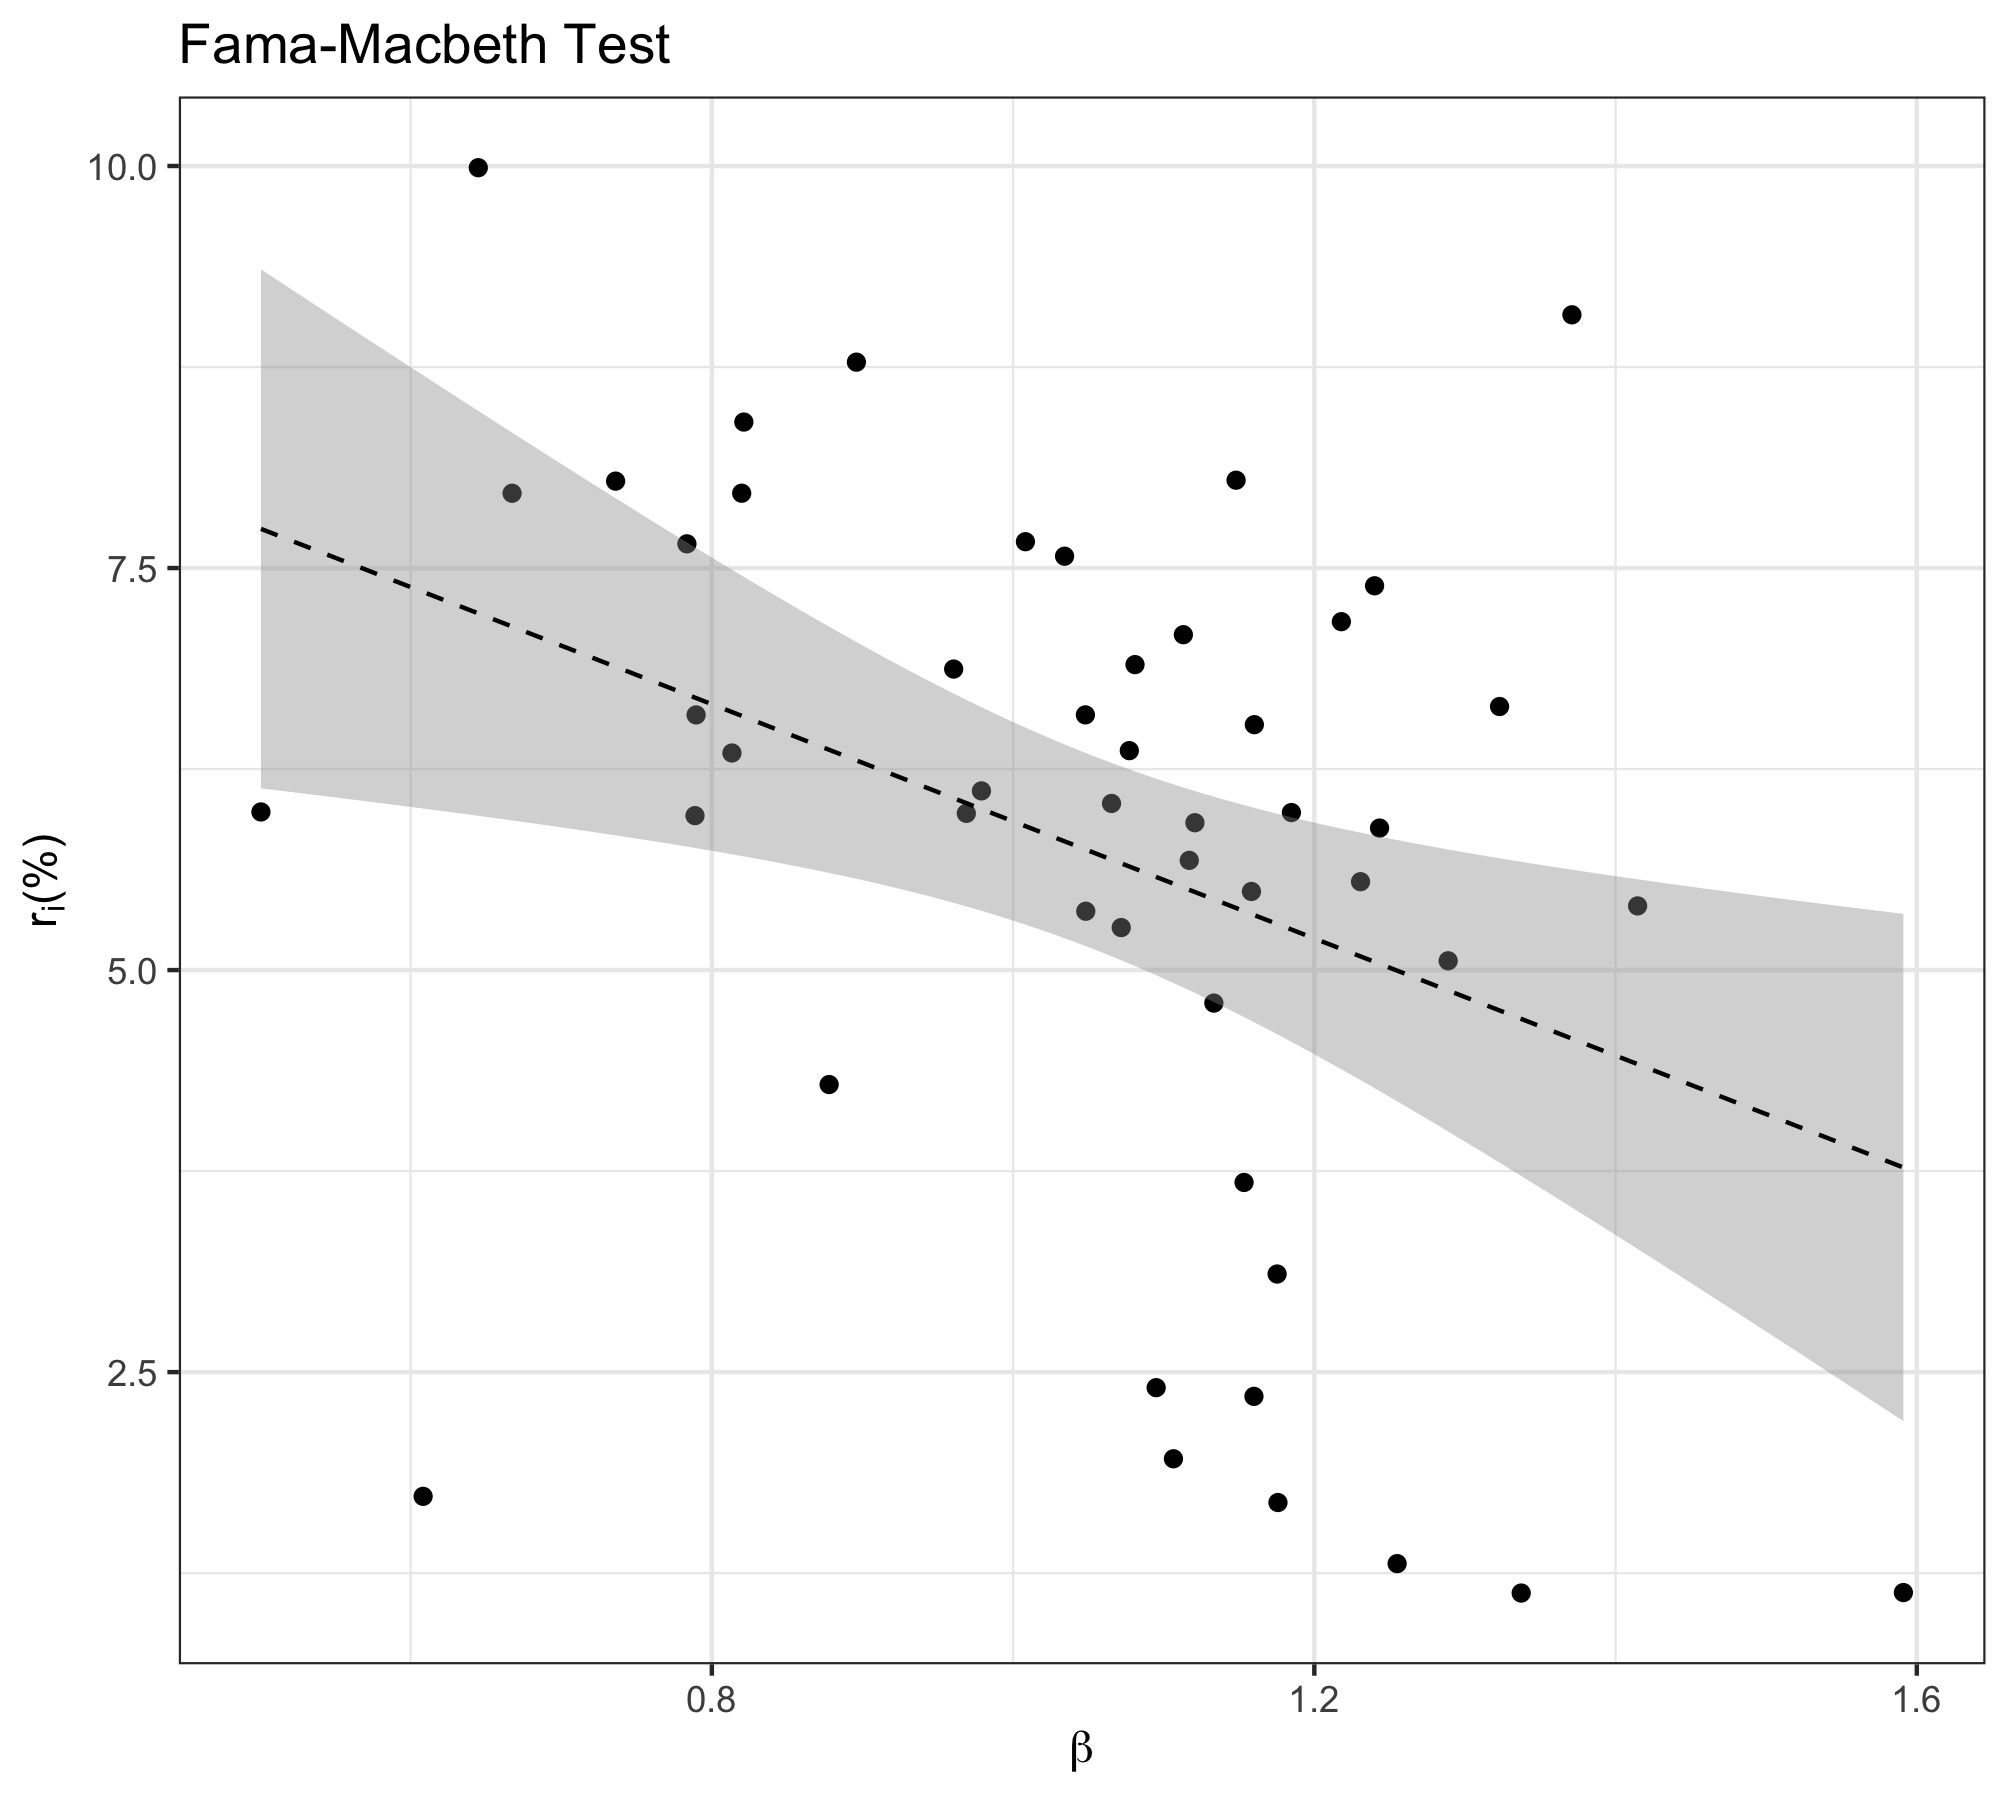
\includegraphics[width=0.5\textwidth]{q2_fmtest.jpg}
	\end{figure}

	If the CAPM held, the relationship between $ r_i $ and $ \beta $ would be positive and linear. Instead, as the fitted line shows, the relationship is somewhat negative. This relationship is not strong; the confidence bands (shaded in grey) around this line are wide. 
		
	\end{enumerate}
		


	\item In this economy, the states are $ s\in\{s_1, s_2\} $, with prices $ P $ and payoffs $ D $ as follows:
	%
	\begin{gather*}
	P = \begin{bmatrix} 1.575 & 1.35 & 3.425 \end{bmatrix}\\ 
	D = \begin{bmatrix} 2 & 1 & 4 \\ 1 & 3 & 3 \end{bmatrix}
	\end{gather*}
	\begin{enumerate}
		\item This setup allows for arbitrage. Intuitively, the number of states is less than the number of assets, and thus one of the assets must be redundant. This intuition is confirmed by noting that a portfolio of $ 9/5 $ asset 1 plus $ 2/5 $ asset 2 delivers identical payoffs to asset 3, while costing
		\[\frac{9}{5}\cdot 1.575 + \frac{2}{5} 3.375 < 3.425 \]
		Thus, an agent can extract unlimited profits by buying $ 9/5 $ asset 1 plus $ 2/5 $ asset 2, and selling asset 3. 
		
		\item Figure \ref{q3_arb} illustrates the arbitrage in this example: \newpage
		
		\begin{figure}[!h]
			\centering
			\caption{}
			\label{q3_arb}
			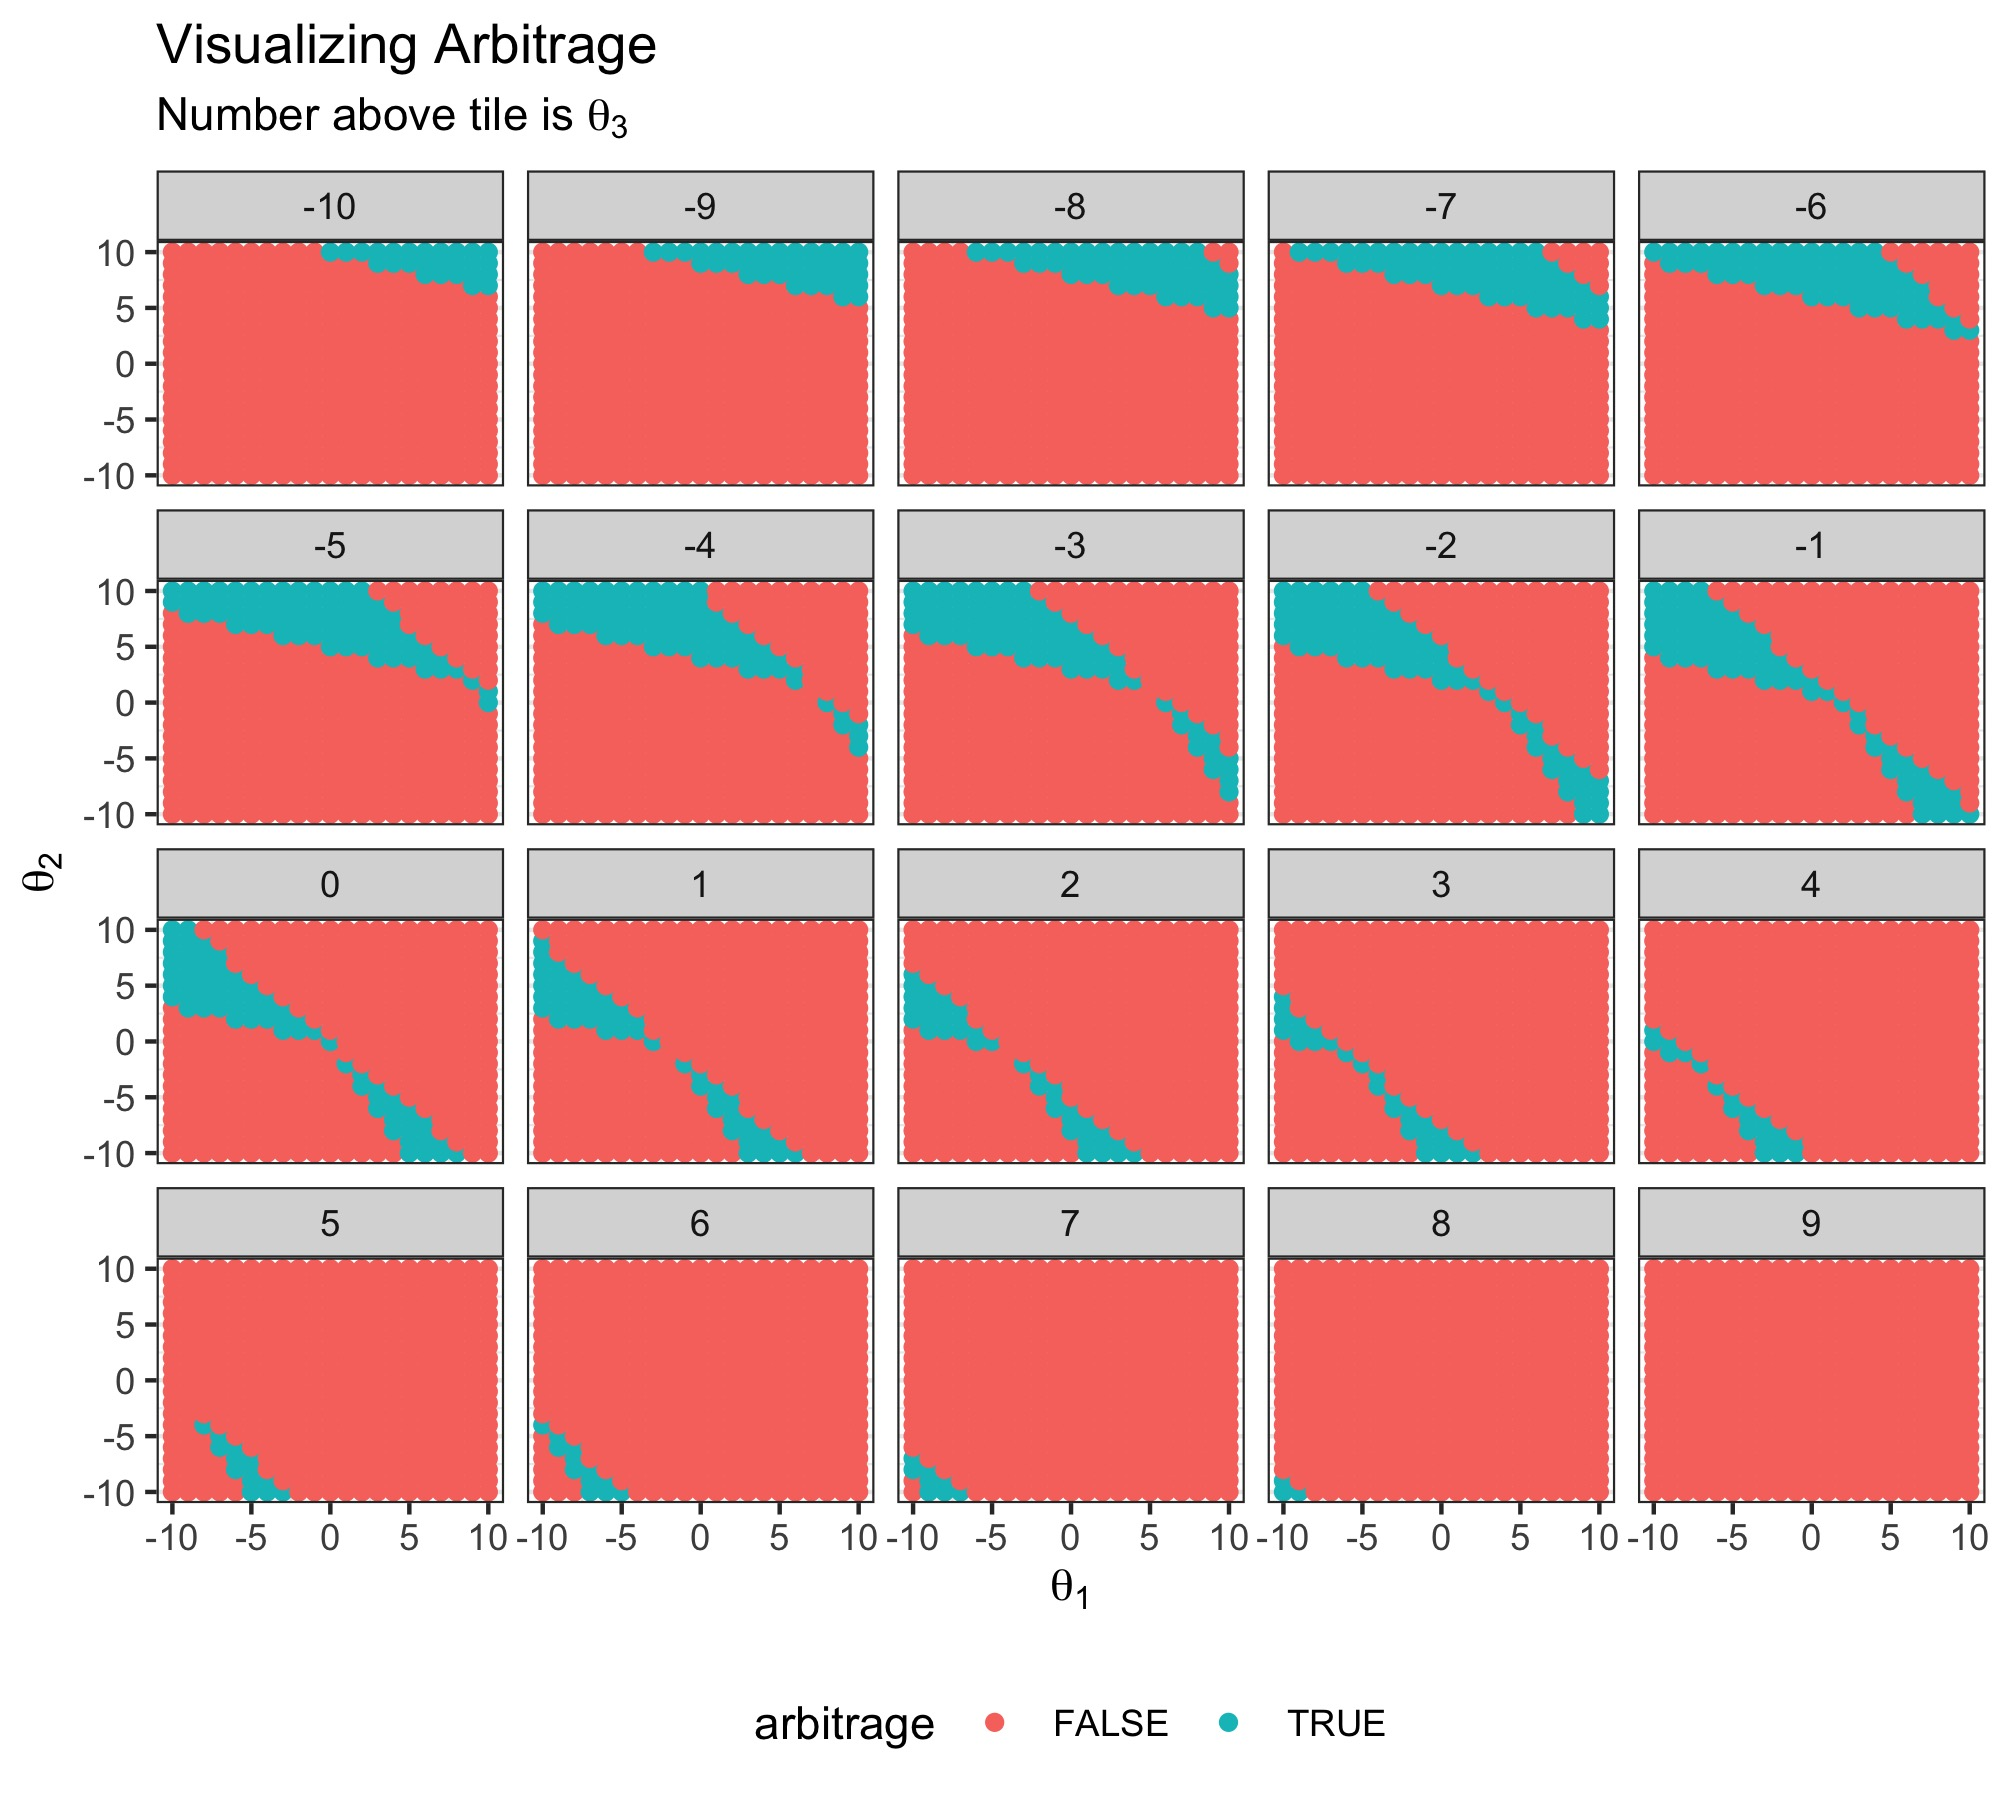
\includegraphics[width=0.7\textwidth]{q3_arb.jpg}
		\end{figure}
		
		In Figure \ref{q3_arb}, the $ x $-axis represents the shares of asset 1, the $ y $-axis the shares in asset 2, and the numbers in shaded gray boxes above the tiles the shares in asset 3. The teal areas are portfolios for which $ P\theta \leq 0 $ and $ D\theta\geq 0 $.
	\end{enumerate}
	
	\item In this economy, there are three states, $ s\in\{s_1, s_2, s_3\} $, each with equal $ 1/3 $ probability. The prices and payoffs are as follows: 
	\begin{gather*}
	P = \begin{bmatrix} 2.4 & 1.248 & 5.952	\end{bmatrix} \\
	D = \begin{bmatrix}
	4 & 1 & 11 \\
	1 & 2 & 1 \\ 
	1 & 1 & 2 \\
	\end{bmatrix}
	\end{gather*}
	\begin{enumerate}
		\item This market is not complete. Row-reducing the matrix $ D $ shows that 
		\[D = \begin{bmatrix}
		1 & 0 & 3 \\ 0 & 1 & -1 \\  0 & 0 & 0
		\end{bmatrix}\]
		Thus, the rank of $ D $ is two, and the span of $ D $ is $ \mathbb{R}^2 $. 
		
		\item With complete markets, the Arrow-Debreu state prices are given by the vector $ A = P\inv{D} $. However, because $ D $ is not of full rank, it cannot be inverted. Thus, there exists a continuum of Arrow-Debreu state prices. Given any $ a(s_3) $, prices $ a(s_1) $ and $ a(s_2) $ can be chosen in order to construct the replicating portfolio. 
		
		\item Because there is a continuum of A-D state prices, there is a continuum of risk-free rates. To see this, note that $ R_f = 1/B $, where $ B = \sum_{s = 1}^k a(s_k) $. Because there is an infinite number of values that any $ a(s) $ can take, there will similarly be a continuum of values for the risk-free rate. 
		
		\item Once again, there is a continuum of values that the risk-neutral probabilities can take, as $ q(s) = a(s)/B$, both of which are undetermined.
		
		\item The pricing kernel $ m(s) = a(s) / p(s)  = 3 a(s) $ can also take an infinite number of values.
		
		\item The date-$ T $ consumption plan $ c_T = (18, 8, 6)^\p $ is attainable. Pricing this consumption plan, however, is complicated due to the incompleteness of the markets. Choosing any nonzero amount of asset three to hold (denoted $\theta_3$), this plan can be financed by any holdings $ (\theta_1, \theta_2, \theta_3) $ such that $ \theta_1 = 4 - 3\theta_3 $ and $ \theta_2 = 2 + \theta_3 $. 
		
		\item The date-$ T $ consumption plan $ c_T = (18, 8, 6)^\p $ is \emph{not} attainable. $ (18, 8, 6)^\p $ is not in the span of $ D $; there is no combination of asset holdings that can finance this plan. The only way to achieve this plan is to have $ c_T $ as one's date-$ T $ endowment. 
		\end{enumerate}
	
		\item Here there are two states, $ s\in\{s_{down}, s_{up}\} $. 
		\begin{enumerate}
			\item With a risk-free rate of $ 1 \% $, and prices $ P = \begin{pmatrix} 1 & 1\end{pmatrix} $, the payoffs on the bond are given by $ \begin{pmatrix}	1.01 & 1.01	\end{pmatrix}^\prime $. 
			
			\item The payoffs for the stock complete the matrix of dividends: 
			\[ D = \begin{bmatrix}
			1.01 & 0.87 \\ 1.01 & 1.27
			\end{bmatrix}\]
			The payoffs to the stock are chosen such that its expected excess return is $ 6\% $, and its standard deviation is about $ 20\% $ per year. 
			
			\item The Arrow-Debreu state prices are as follows:
			\[A = \begin{bmatrix} a(s_{down}) \\ a(s_{up})\end{bmatrix} = \begin{bmatrix} 0.644 \\ 0.347 \end{bmatrix}\]
			
			\item The risk-neutral probabilities are 
			\[q = \begin{bmatrix}
			0.65 \\ 0.35
			\end{bmatrix}\]
			
			\item The pricing kernel $ m $ is given by 
			\[m = \begin{bmatrix}
			1.287 \\ 0.693
			\end{bmatrix}\]
			
			\item Figure \ref{fig_q5} shows how the pricing kernel changes in response to $\mu$ and $\sigma$. Figures \ref{fig1_a} and \ref{fig1_b} show that the ratio $ m(s_{down}) / m(s_{up}) $, as well as the standard deviation $\sigma_m$, increase in $\mu$. Figures \ref{fig1_c} and \ref{fig1_d}, meanwhile, show that the ratio and $\sigma_m$ decrease as the variance $\sigma$ increases. 
			
			\newpage
			\begin{figure}[!hbt]
				\caption{}
				\begin{subfigure}{.5\textwidth}
					\centering
					\caption{Pricing Kernel Ratio as function of $\mu$}
					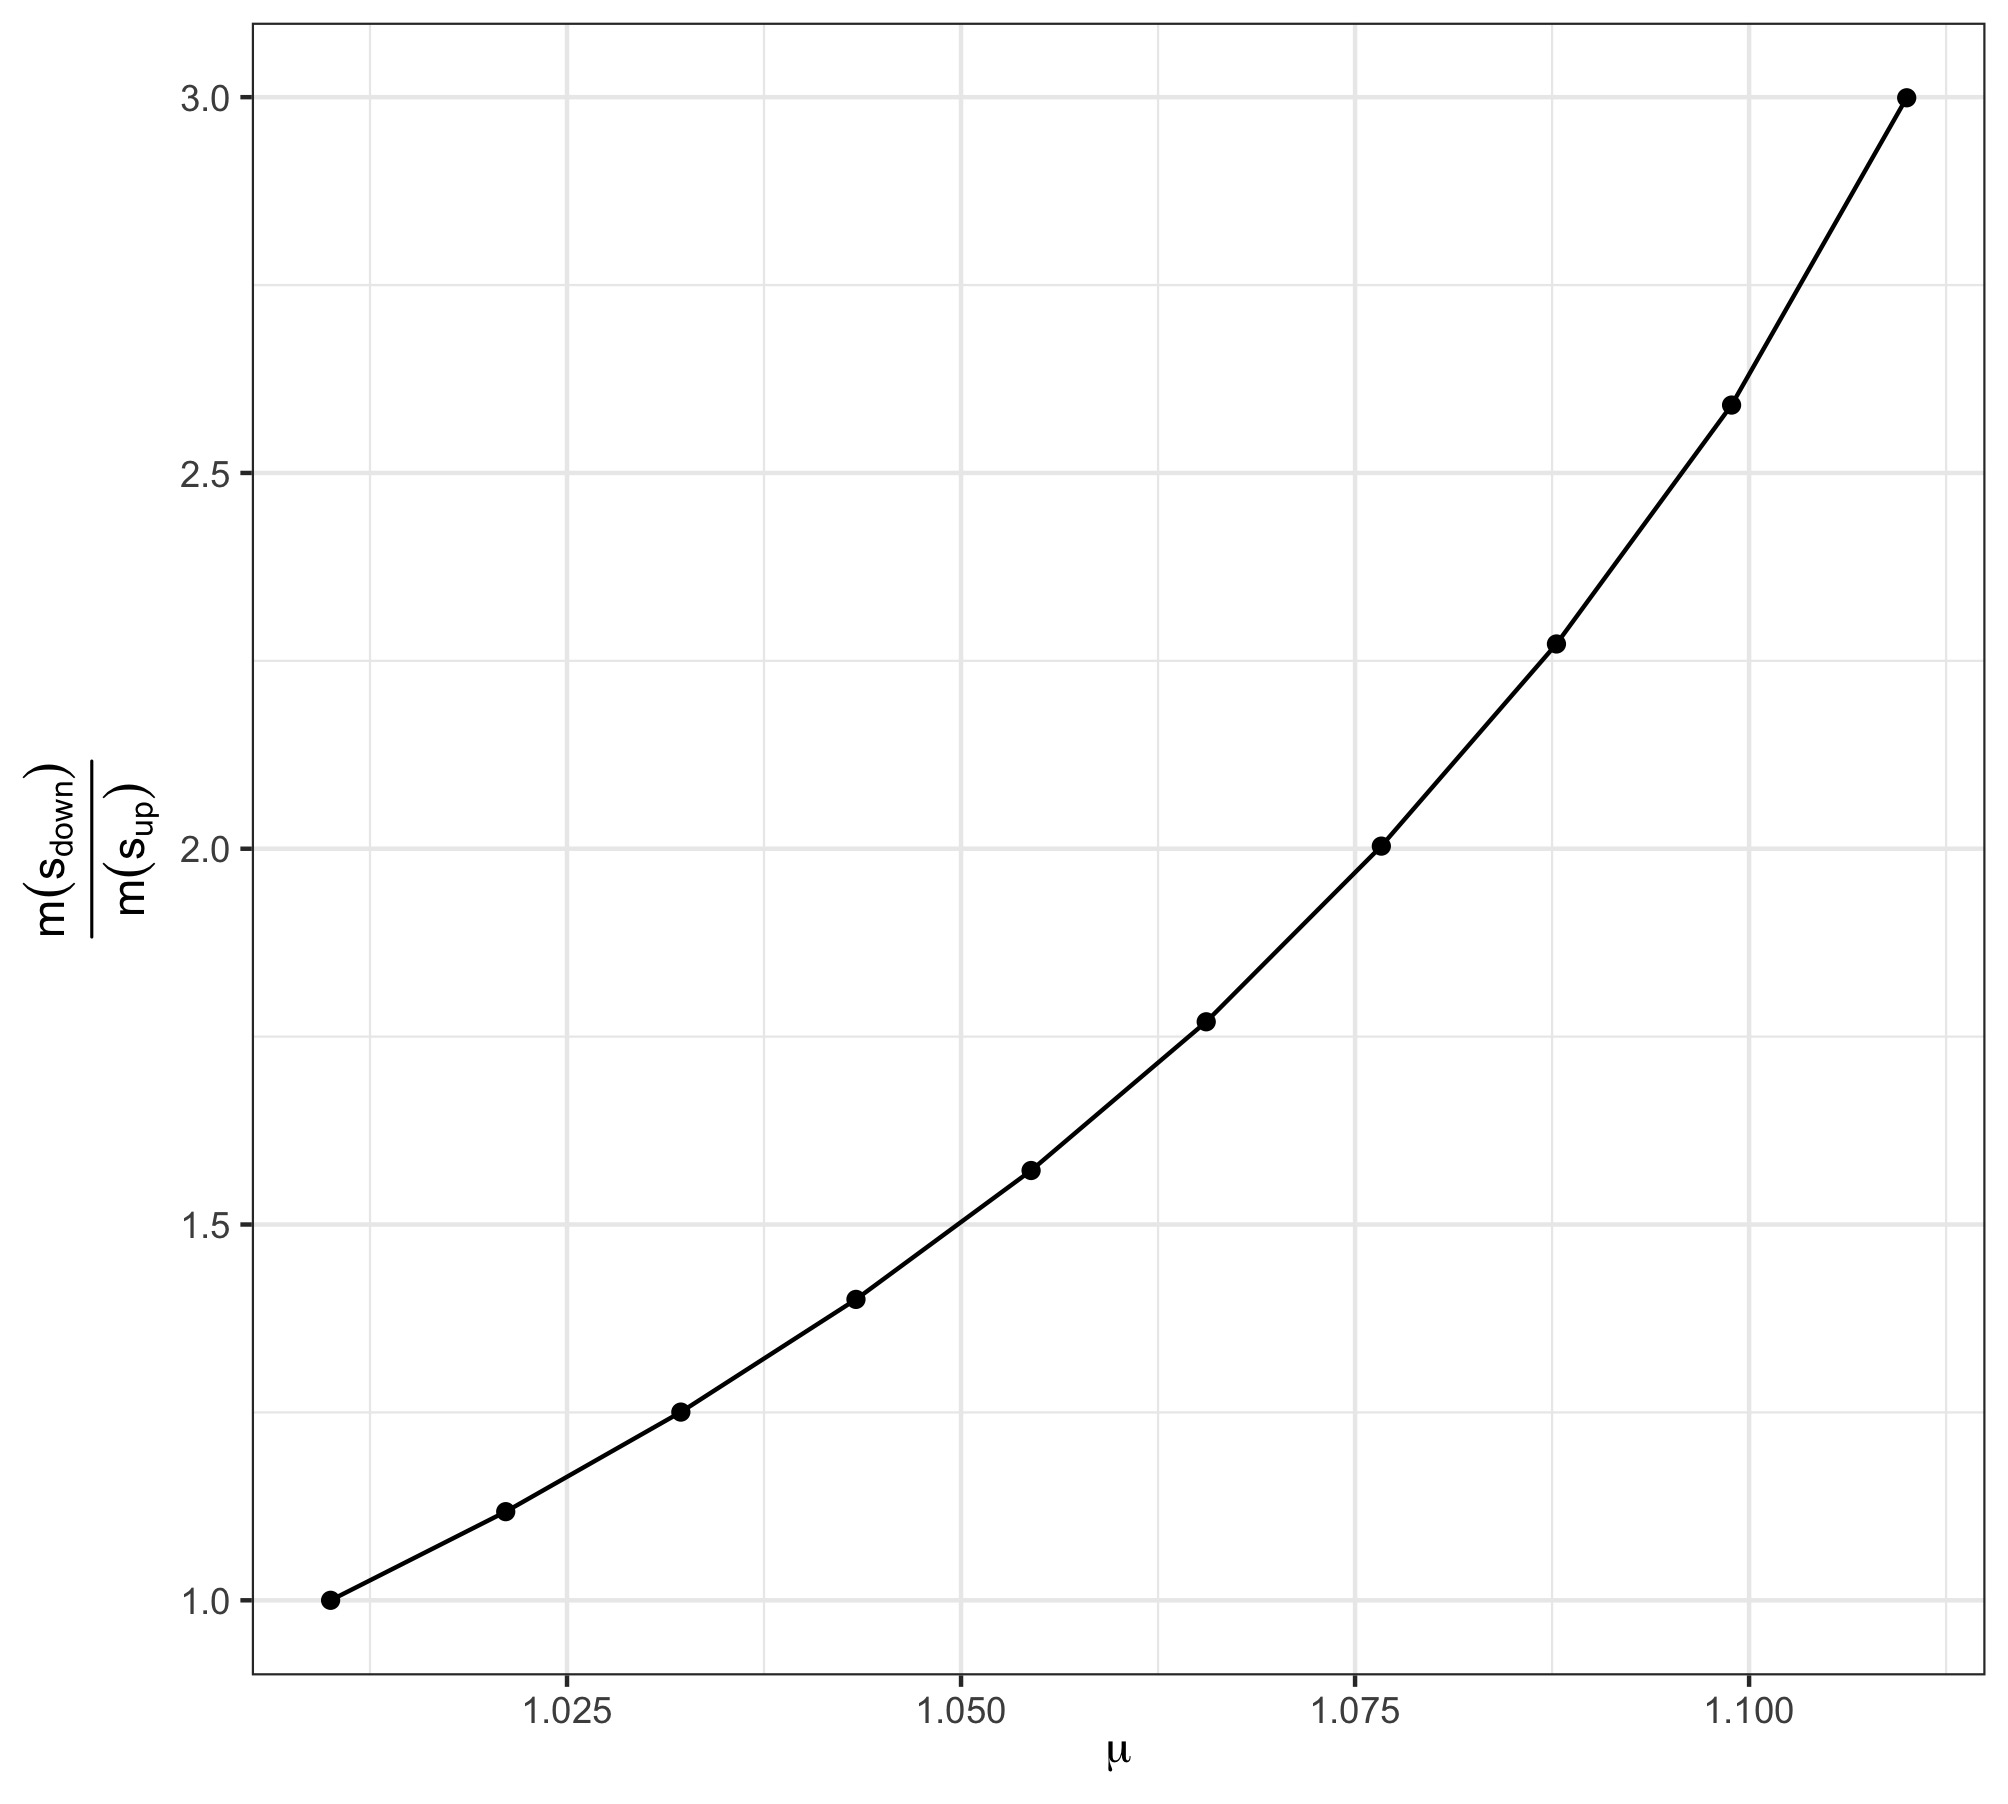
\includegraphics[width=.8\linewidth]{q5_fig1}
					\label{fig1_a}
				\end{subfigure}%
				\begin{subfigure}{.5\textwidth}
					\centering
					\caption{$\sigma_m$ as function of $\mu$}
					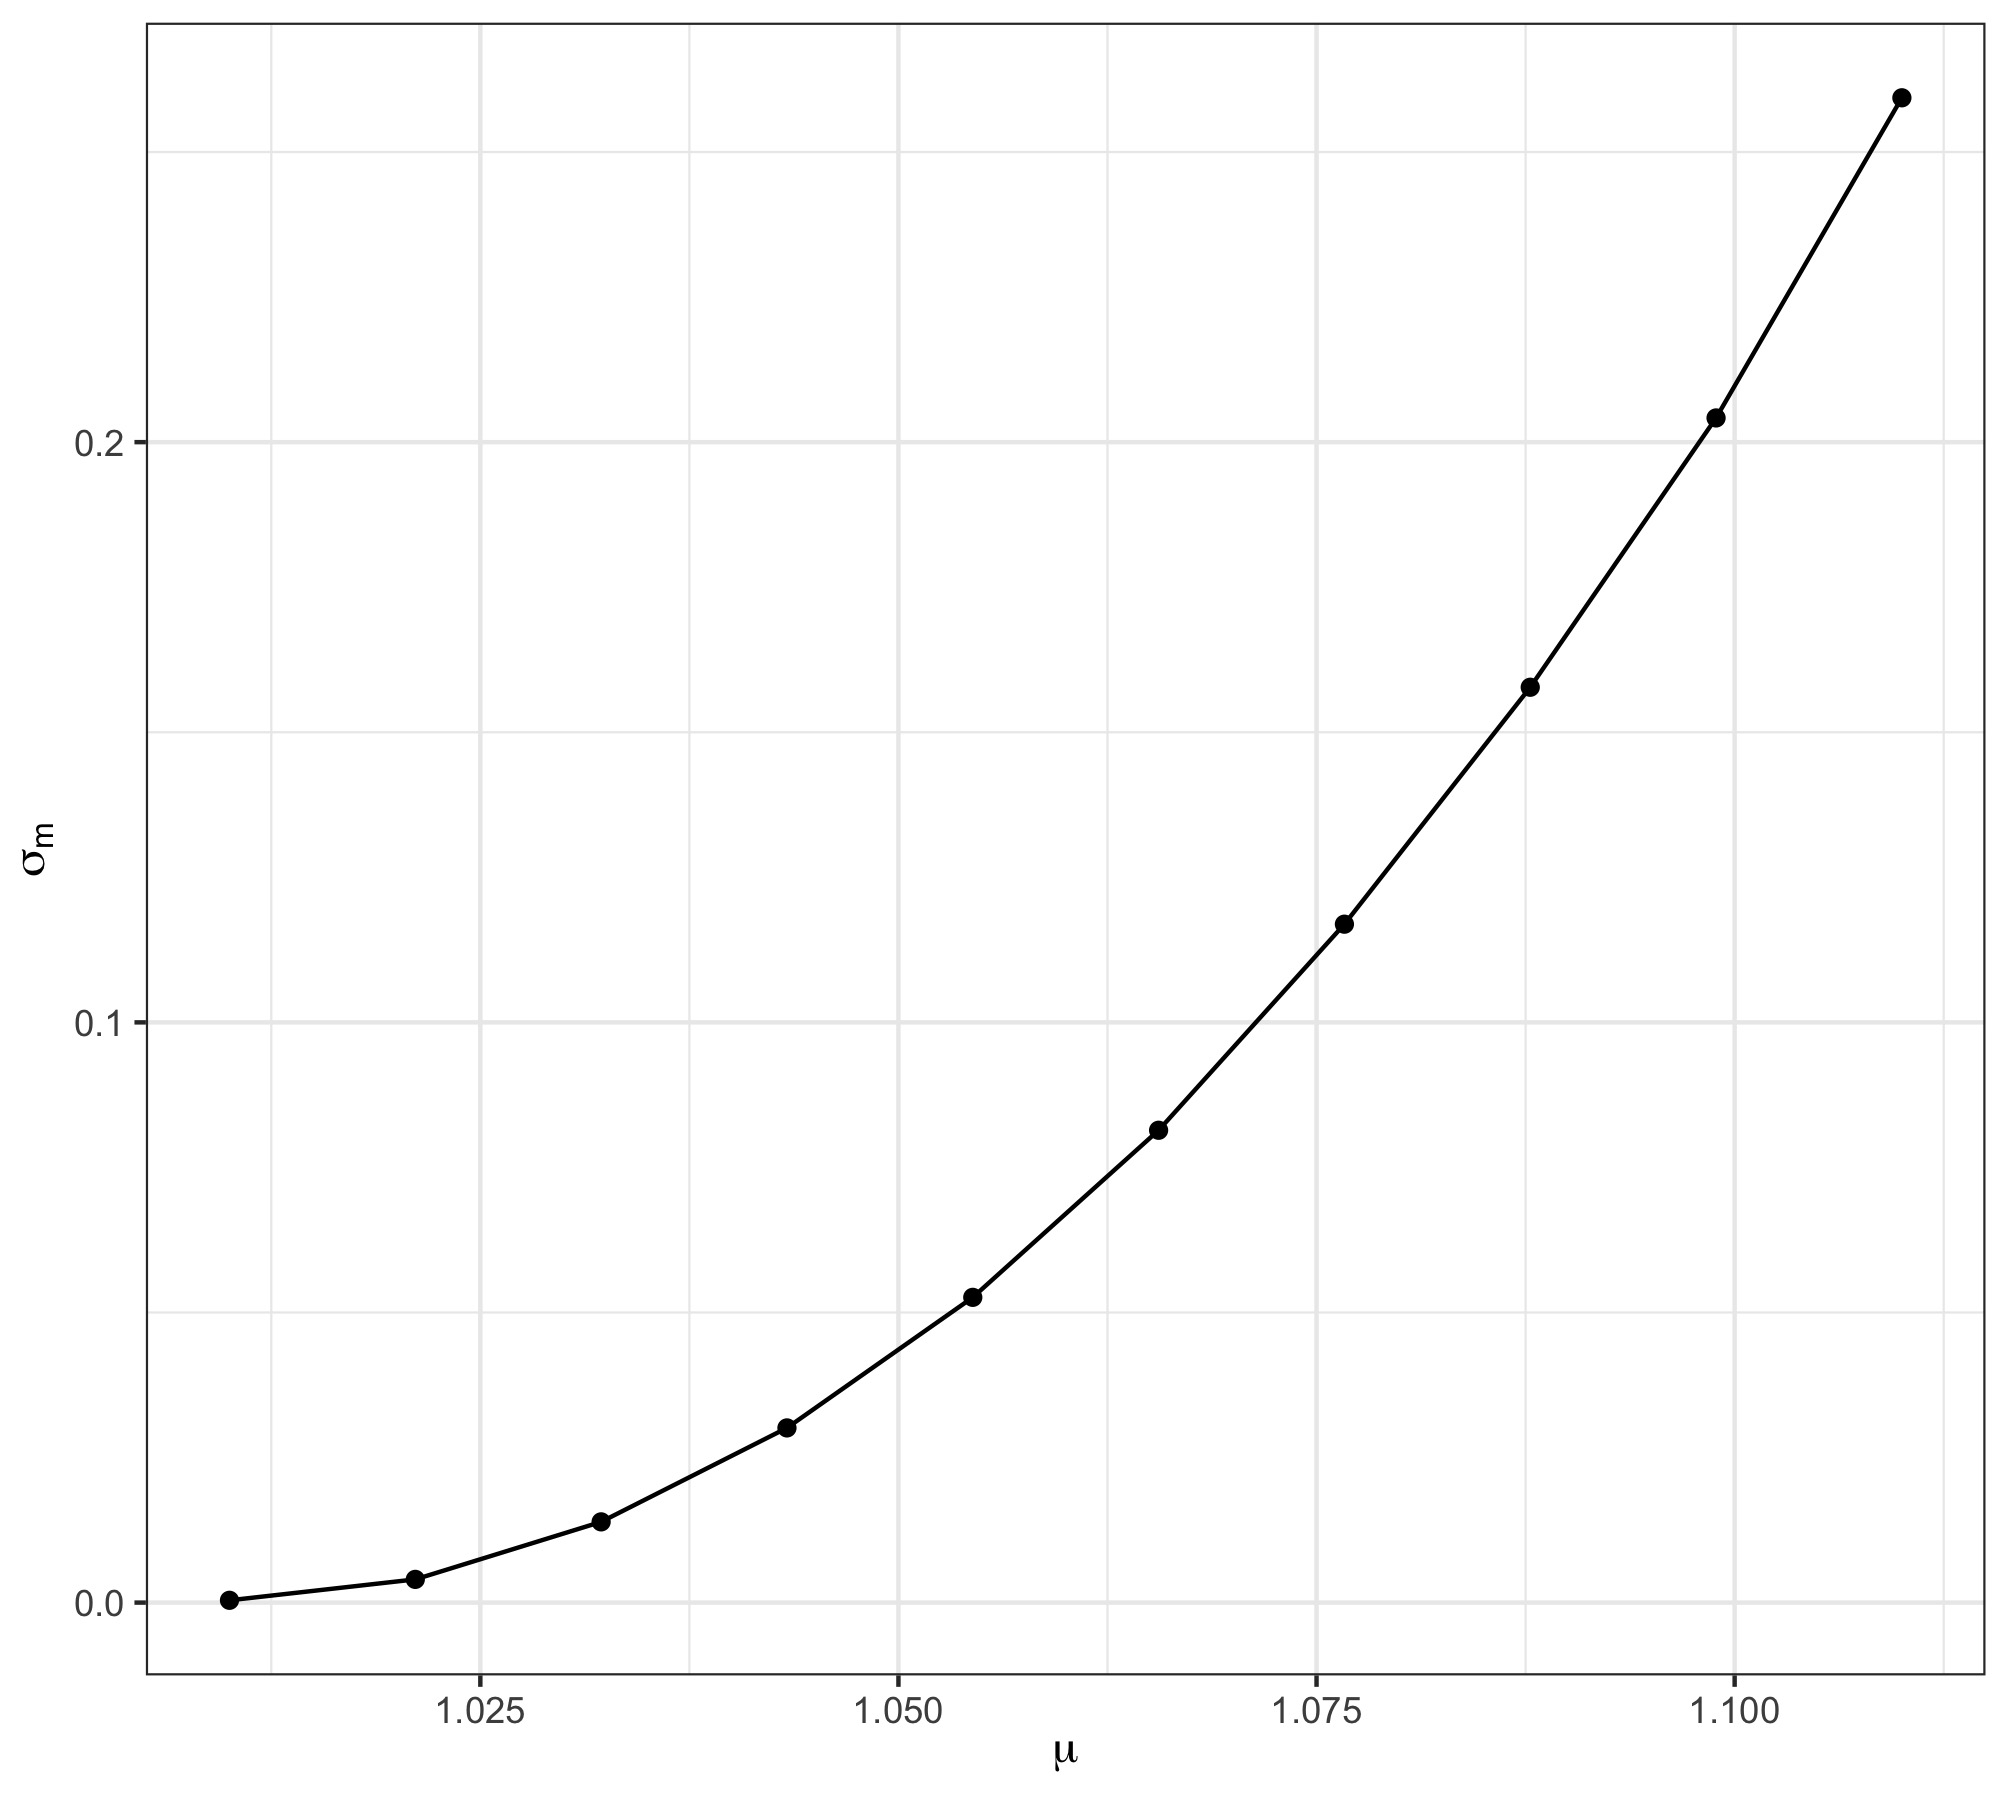
\includegraphics[width=.8\linewidth]{q5_fig2}
					\label{fig1_b}
				\end{subfigure}
				\begin{subfigure}{.5\textwidth}
					\centering
					\caption{Pricing Kernel Ratio as function of $\sigma$}
					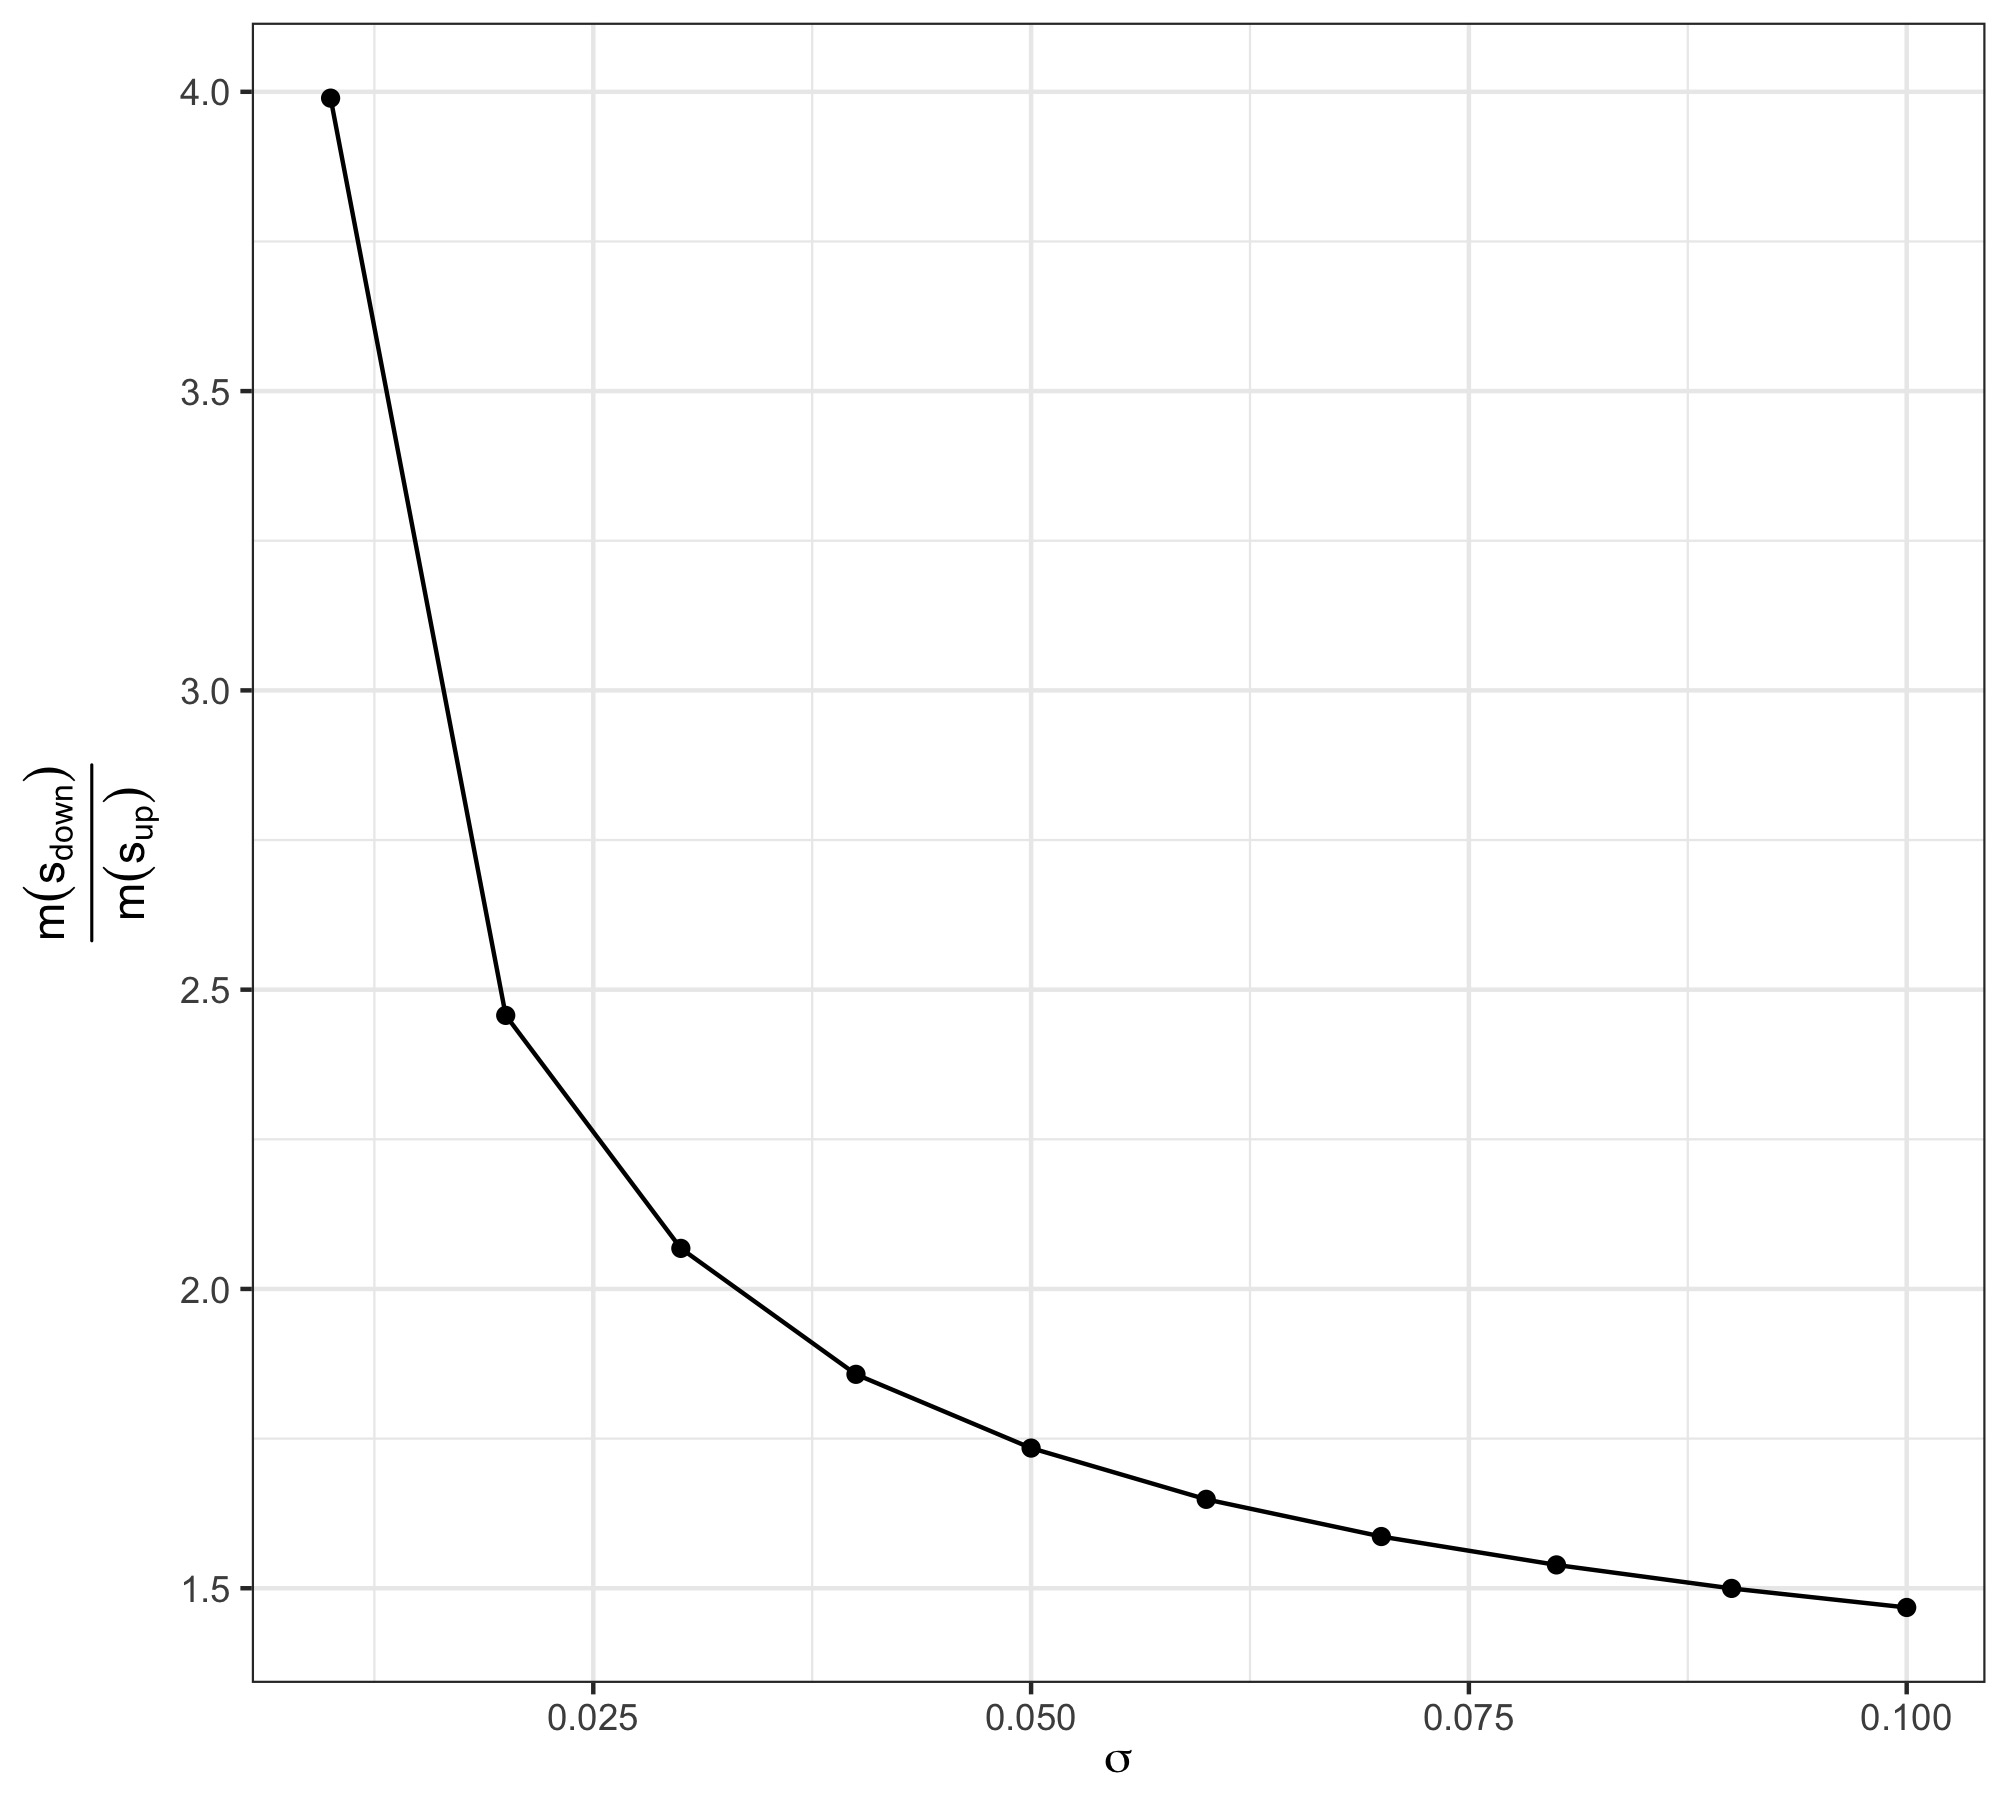
\includegraphics[width=.8\linewidth]{q5_fig3}
					\label{fig1_c}
				\end{subfigure}%
				\begin{subfigure}{.5\textwidth}
					\centering
					\caption{$\sigma_m$ as function of $\sigma$}
					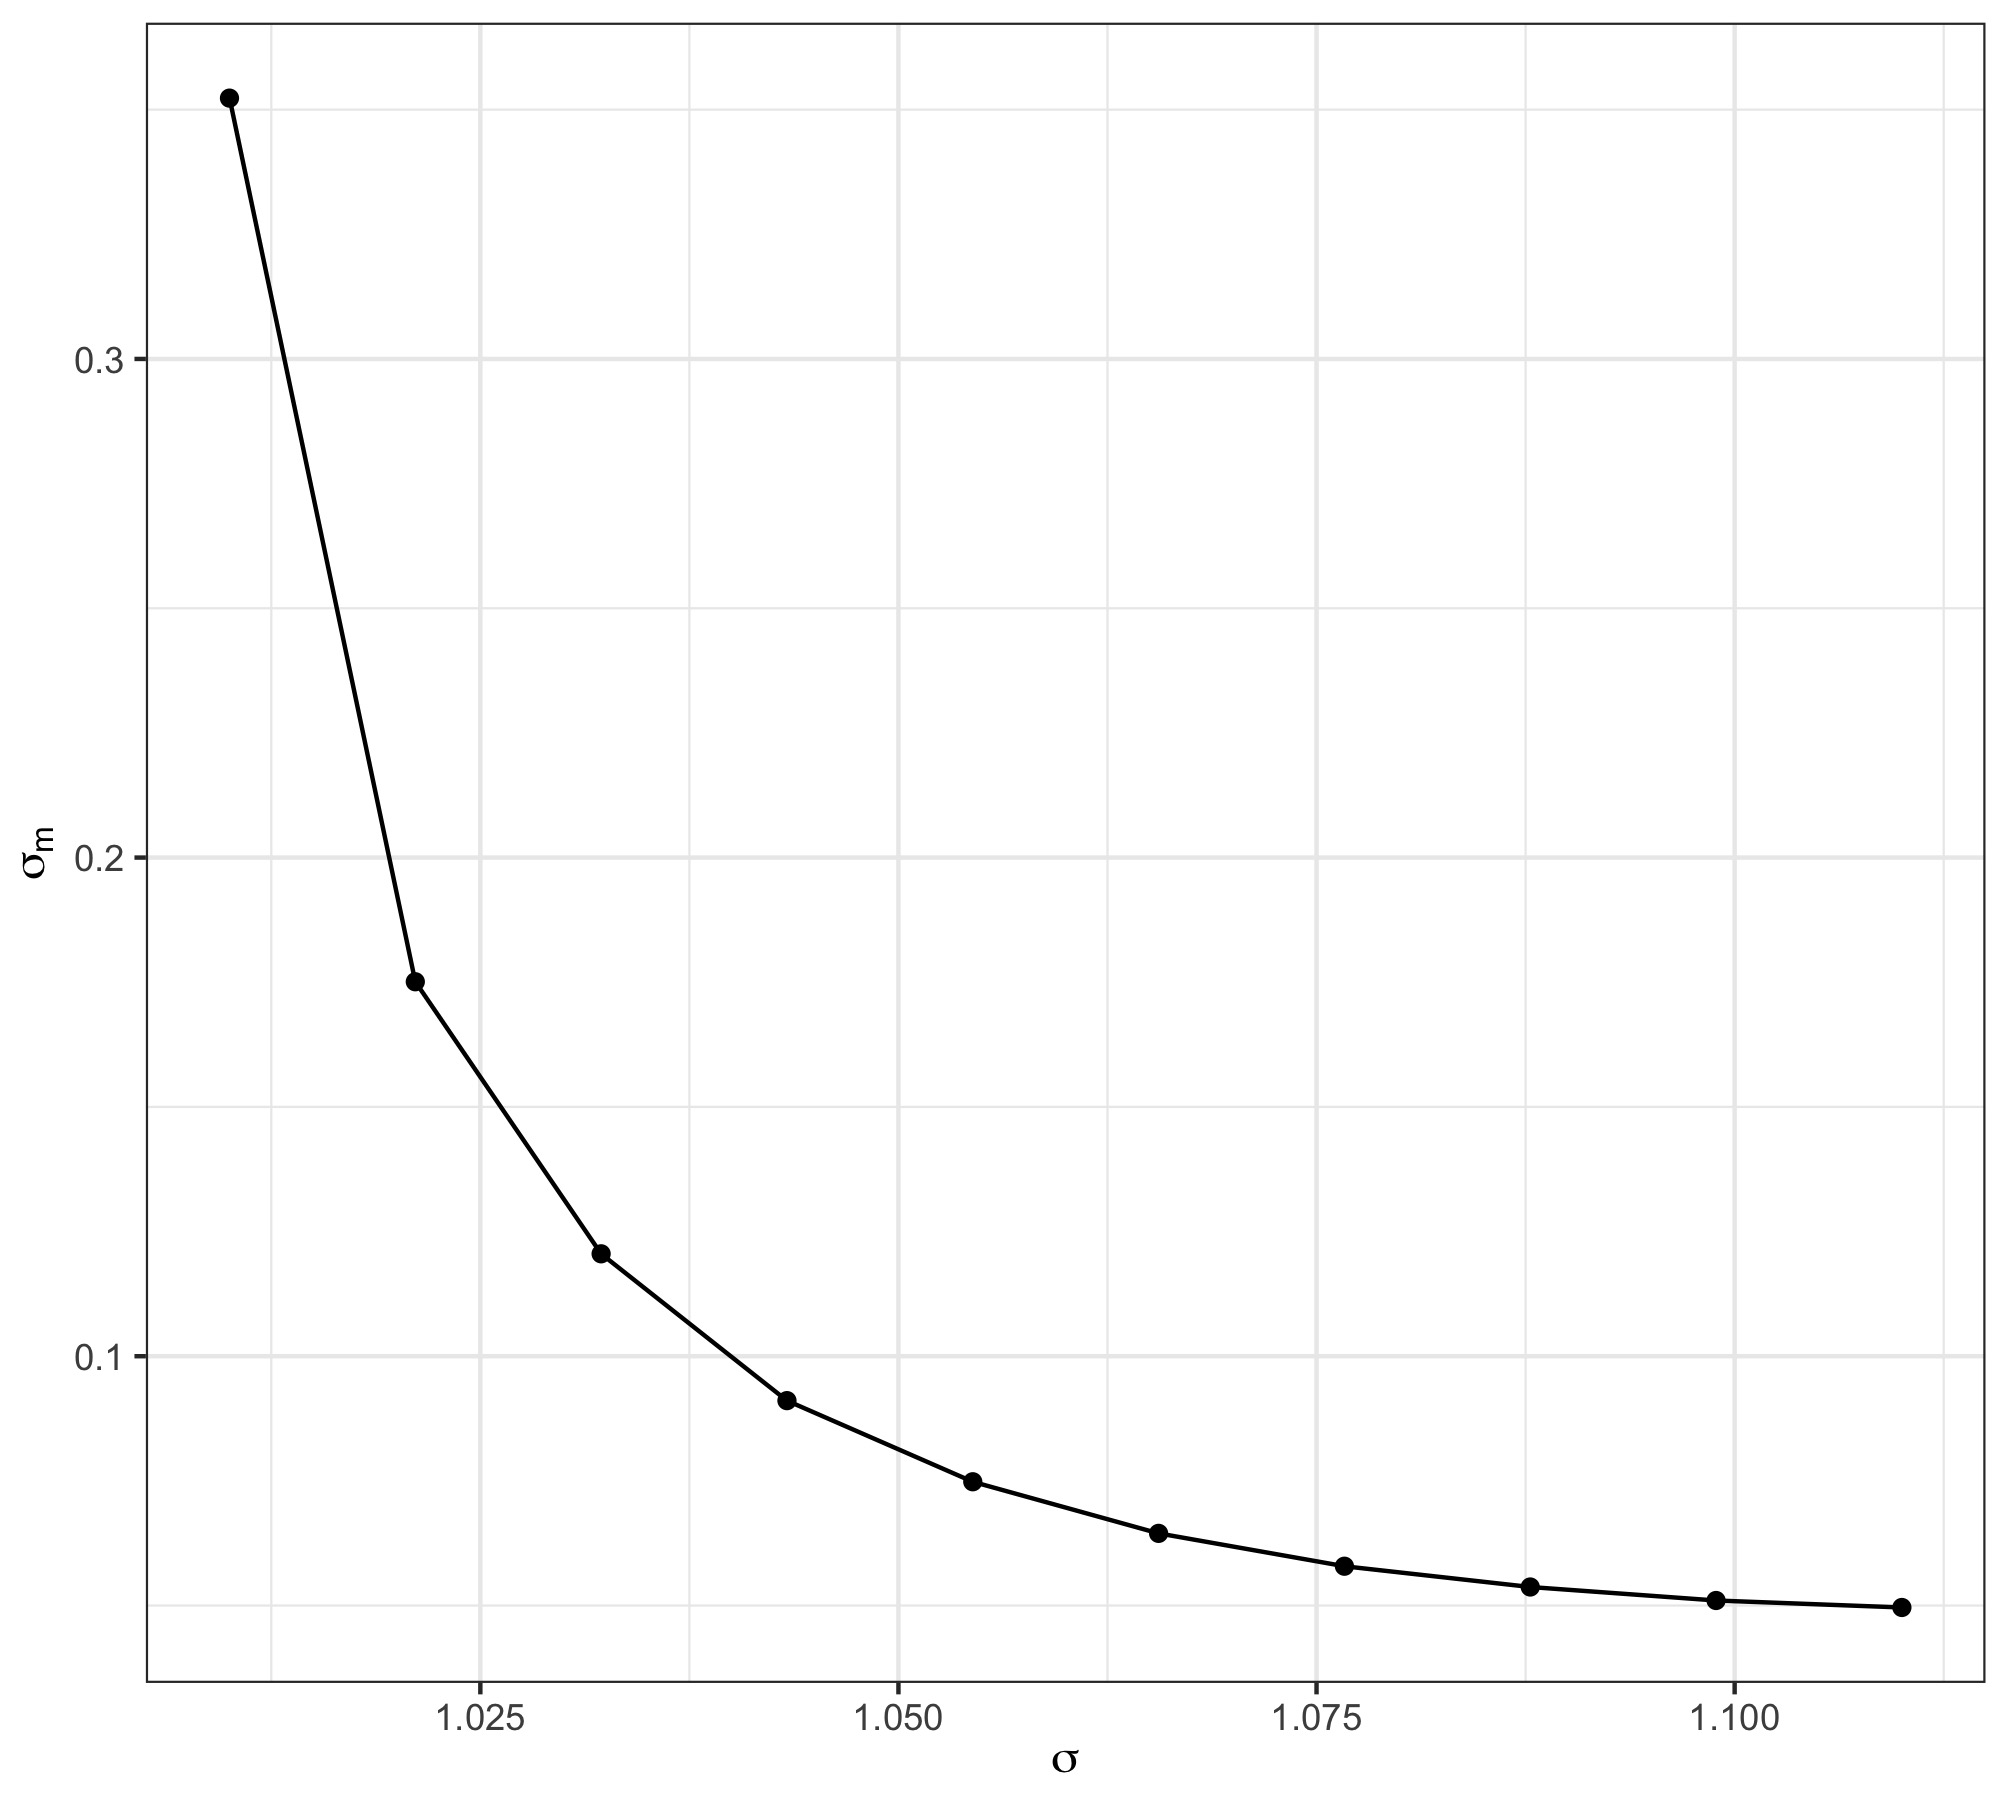
\includegraphics[width=.8\linewidth]{q5_fig4}
					\label{fig1_d}
				\end{subfigure}
				\label{fig_q5}
			\end{figure}
		\end{enumerate}
		
		\item \begin{enumerate}
			\item Figure \ref{q6_fig1} shows the efficient frontier for two industries, Agriculture and business services:
			
			\begin{figure}[!ht]
				\centering
				\caption{}
				\label{q6_fig1}
				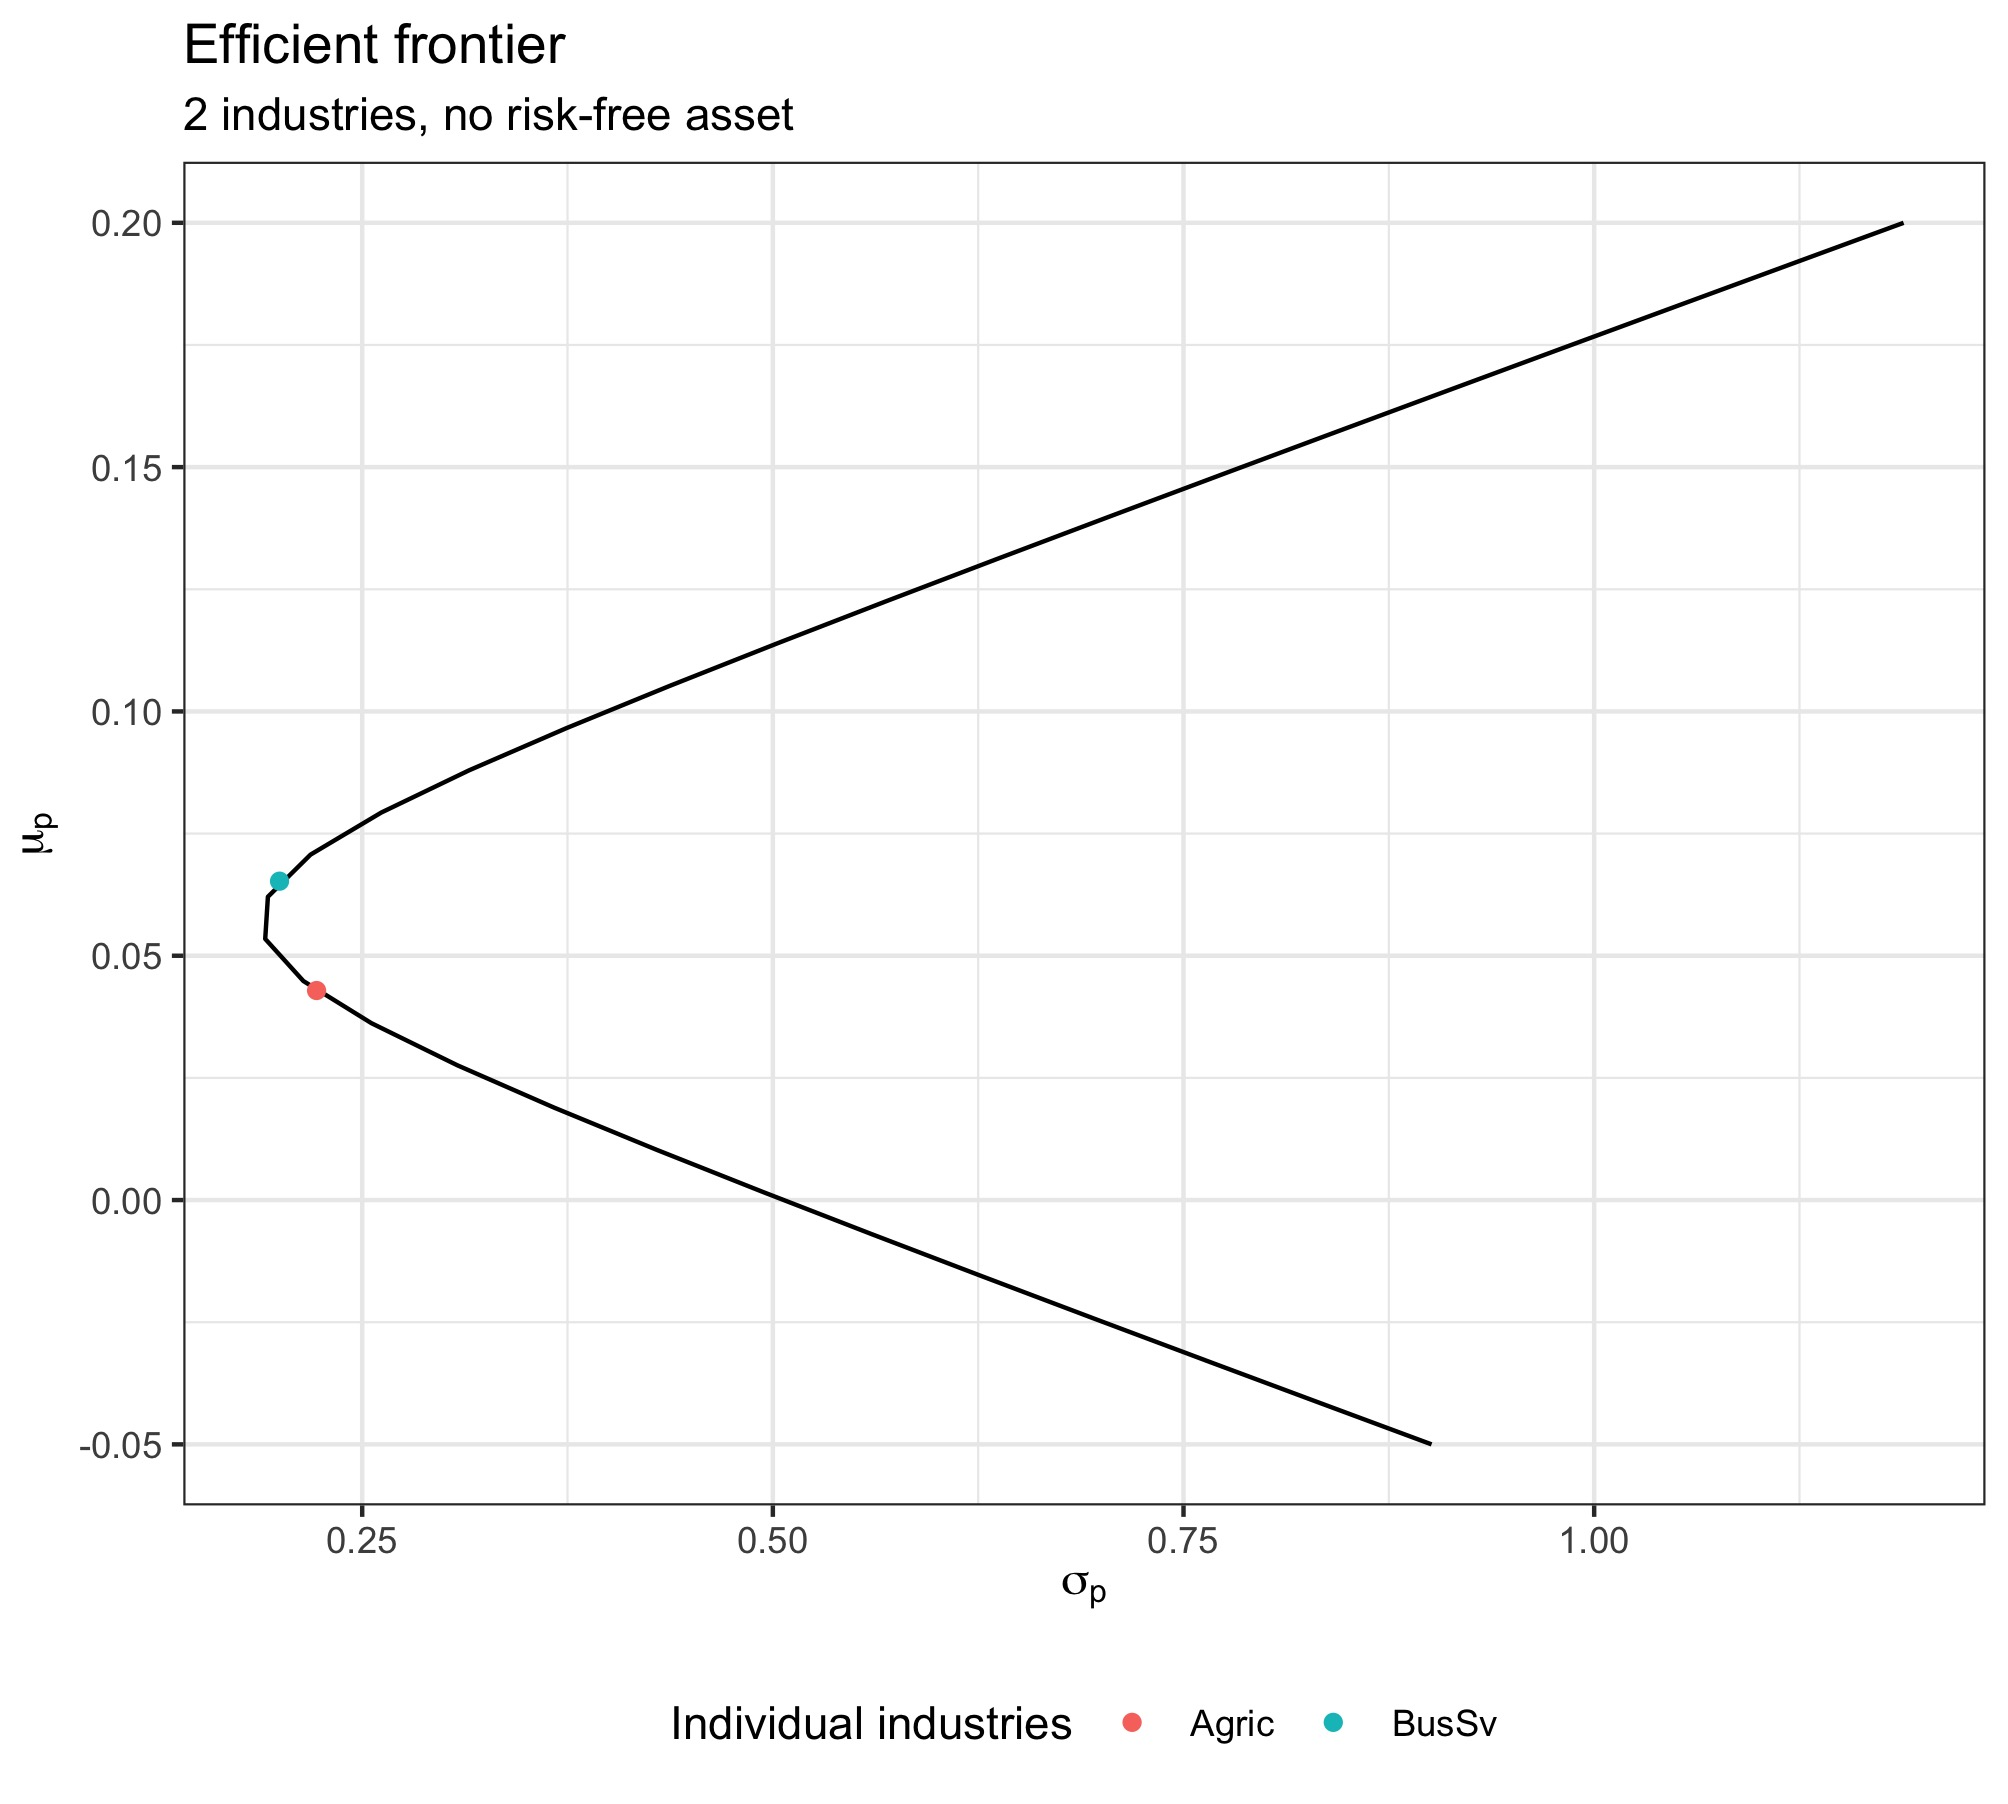
\includegraphics[width=0.5\textwidth]{q6_eff_front}
			\end{figure}
			
			\item Table \ref{q6_table} shows the Sharpe Ratio of the portfolio of these two industries selected to maximize this ratio, as well as the Hansen-Jaganathan bound on $\sigma_m$ for each of the Sharpe ratios: \newpage
			
			\begin{table}[!htbp] \centering 
				\caption{} 
				\label{q6_table} 
				\begin{tabular}{@{\extracolsep{5pt}} ccc} 
					\\[-1.8ex]\hline 
					\hline \\[-1.8ex] 
					$ R_f $ & Sharpe Ratio$ _{max} $ & HJ Bound \\ 
					\hline \\[-1.8ex] 
					$1.010$ & $0.279$ & $0.276$ \\ 
					$1.020$ & $0.232$ & $0.227$ \\ 
					$1.030$ & $0.189$ & $0.183$ \\ 
					$1.040$ & $0.152$ & $0.146$ \\ 
					$1.050$ & $0.128$ & $0.122$ \\ 
					\hline \\[-1.8ex] 
				\end{tabular} 
			\end{table} 
		
			\item Figure \ref{q6_fig2} shows the H-J Bound for $ \sigma_m $ as a function of $ \ev[m] $: 
			\begin{figure}[!htbp]
				\centering
				\caption{Hansen-Jaganathan Bound increases in $ \ev[m] $}
				\label{q6_fig2}
				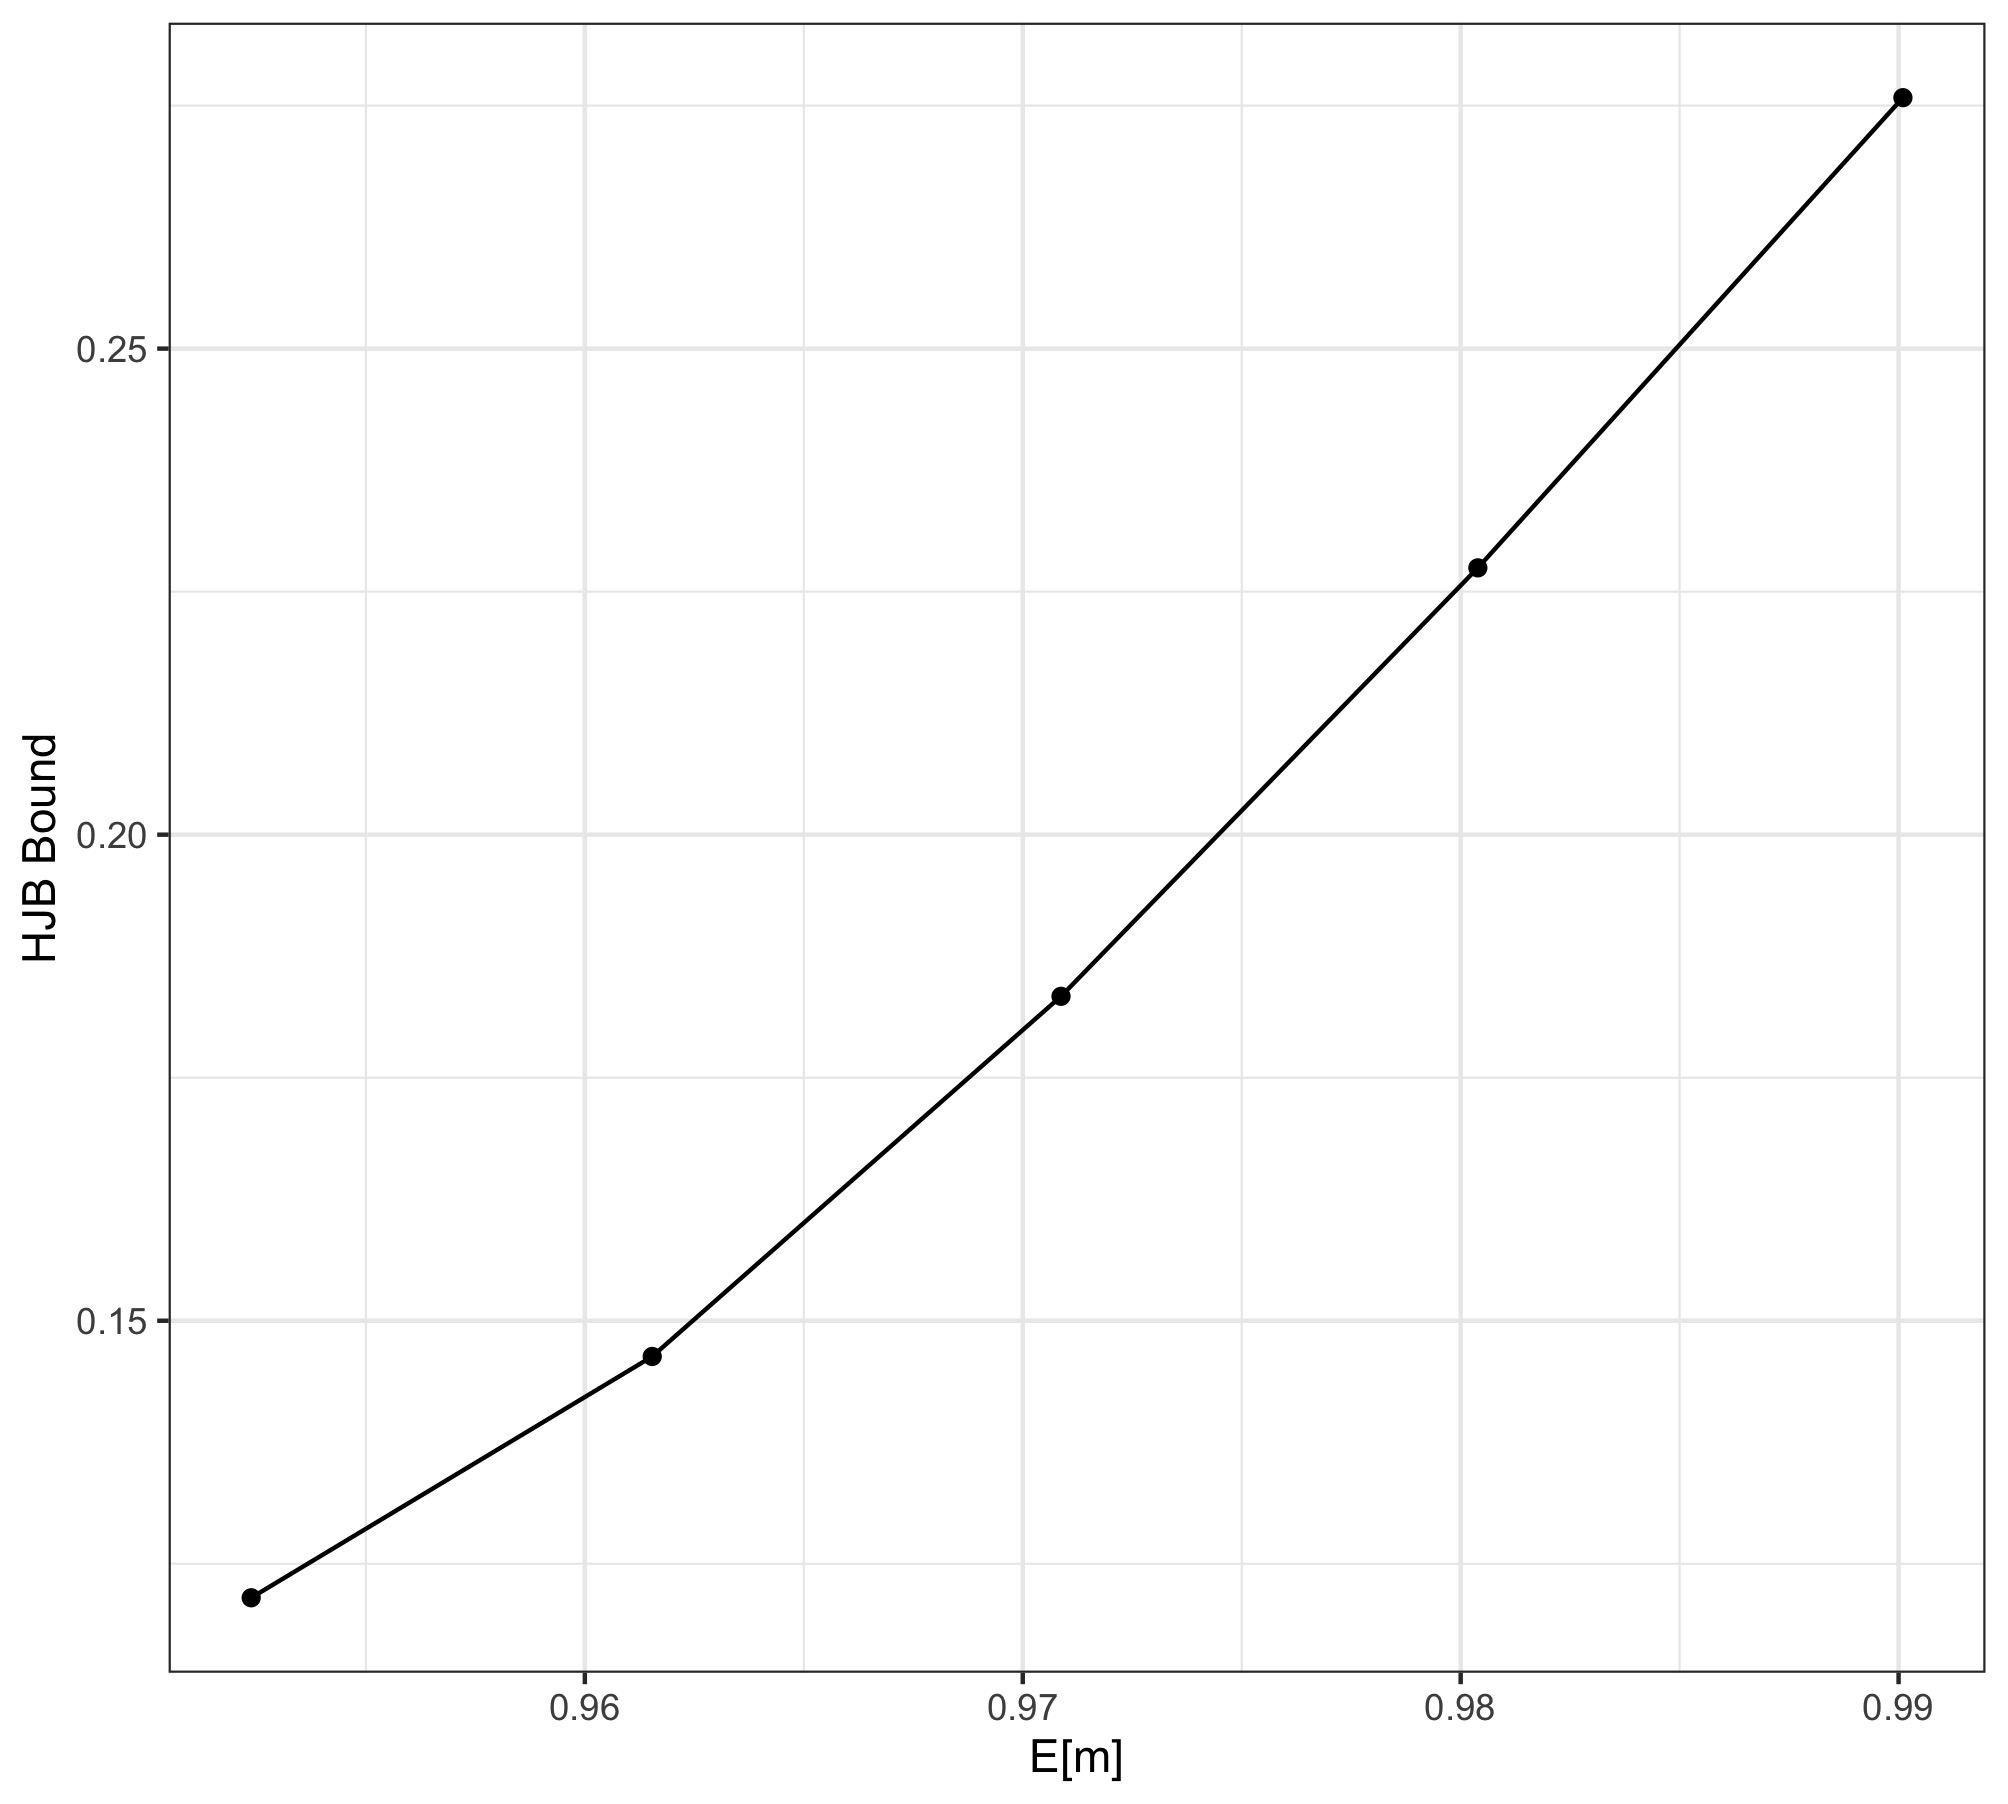
\includegraphics[width=0.5\textwidth]{q6_hjb}
			\end{figure}
		\end{enumerate}
		
		\item The ``Kelly Criterion'' aims to maximize expected log return. Here, we consider solving this criterion, subject to there being no arbitrage; that is,
		\begin{gather*}
		\max_{\{R(s)\}} \ev_t[\log R(s)] \\ 
		\text{s.t.}\quad \ev_t[m(s) R(s)] = 1
		\end{gather*}
		\begin{enumerate}
			\item \cite{alvarez2005using} establish a bound on the result:
			\[\ev_t[m(s) R(s)] = 1 \implies \log \ev_t[m(s) R(s)] = 0\]
			Then, by Jensen's inequality, because the logarithm is a concave function,
			\[\log \ev_t[m(s) R(s)] \geq \ev_t[\log m(s) R(s)]\]
			Combining the two gives 
			\[\ev_t[\log m(s) R(s)] \leq 0 \implies	\ev_t[\log m(s) + \log R(s)] \leq 0 \]
			and thus
			\begin{equation}\label{q7_result1}
			\ev_t[\log R(s)] \leq -\ev_t[\log m(s)]
			\end{equation}
			
			\item Continuing from the result in part (a), \cite{alvarez2005using} proceed as follows: 
			\begin{align*}
			L_t(m(s)) &\equiv \log\ev_t m(s) - \ev_t \log m(s) \\
			&= -\ev_t[\log m(s)] - \log R_f \\
			&\geq \ev_t[\log m(s)] - \log R_f \\
			&= \ev_t[\log R(s) - \log R_f]
			\end{align*}
			where the inequality is exactly (\ref{q7_result1}). 
			
			\item The Hansen-Jaganathan bound, meanwhile, is defined as follows. Beginning with the no arbitrage condition,
			\[\ev[m(R_n - R_f)] = 0\]
			which implies that
			\[\ev[m]\ev[R_n - R_f] + cov(Rn - R_f, m) = 0\]
			This further implies that
			\[\frac{\ev[m]\ev[Rn - R_f]}{\sigma_m \sigma_n} + \rho(R_n - R_f, m) = 0\]
			where $ \rho $ is the correlation. Rearranging:
			\[\frac{\ev[m]\ev[Rn - R_f]}{\sigma_n} = -\rho(R_n - R_f, m)\sigma_m\]
			and thus finally,
			\[\frac{\ev[Rn - R_f]}{\sigma_n} \leq \frac{\sigma_m}{\ev[m]}\]
			
			If $ \log m \sim NID(\bar{m}, \sigma_m^2) $ and $ \log R_n^j \sim NID(\bar{r}_n, \sigma_n^2) $, then the Alvarez-Jermann Bound becomes
			\[\log R_f - \exp(\bar{m} + \frac{\sigma_m^2}{2}) \geq \exp(\bar{r} + \frac{\sigma_n^2}{2})\]
			while the Hansen-Jaganathan bound becomes
			\[\frac{\sigma_m}{\exp(\bar{m} + \frac{\sigma_m^2}{2})} \geq \frac{\ev[R_n - R_f]}{\sigma_n} \approx \sigma_n\]
			In both cases, the variance in the pricing kernel $ m $ serves as a bound for the variance of the portfolio of assets. 
		\end{enumerate} 
		
\end{enumerate}

\bibliographystyle{named}
\bibliography{02_assign}

\end{document}